% !TEX TS-program = pdflatex
% !TEX encoding = UTF-8 Unicode

% This file is a template using the "beamer" package to create slides for a talk or presentation
% - Talk at a conference/colloquium.
% - Talk length is about 20min.
% - Style is ornate.

% MODIFIED by Jonathan Kew, 2008-07-06
% The header comments and encoding in this file were modified for inclusion with TeXworks.
% The content is otherwise unchanged from the original distributed with the beamer package.

\documentclass[1pt]{beamer}
\usefonttheme[onlymath]{serif}
\usepackage{media9}
% \usepackage{beamerthemeshadow}
\usepackage[slovene]{babel}
% or whatever
\setbeamercovered{transparent}
\usepackage{caption}
\captionsetup[figure]{labelformat=empty}% redefines the caption setup of the figures environment in the beamer class.
\usepackage{lmodern}
\usepackage{bm}
\usepackage{units}
\usepackage[utf8]{inputenc}
\usepackage{amsmath}
\usepackage[export]{adjustbox}
% \usepackage{fullpage}
\usepackage{mathrsfs}
\usepackage{amsfonts}
\usepackage{amssymb}
\usepackage{fancyhdr}
\usepackage{mathtools}
\usepackage{color}
\usepackage{tikz}
\newcommand{\Tr}{\mathop{\rm Tr}}
\newcommand{\iu}{{i\mkern1mu}}
\newcommand{\bra}[1]{\langle #1 \vert}
\newcommand{\ket}[1]{\vert#1\rangle}
\newcommand{\avg}[1]{\left\langle#1\right\rangle}
\newcommand{\norm}[1]{\left\Vert #1 \right\Vert}
\newcommand{\braket}[2]{\left\langle #1 \vert#2 \right\rangle}
\newcommand{\obraket}[3]{\left\langle #1 \vert #2 \vert #3 \right \rangle}
\usepackage{times}
% \usepackage[utf8]{fontenc}
\newcommand{\dd}{\,\mathrm{d}}
\newcommand{\ddd}{\mathrm{d}}
\newcommand{\ii}{\mathrm{i}}
\usepackage{mhchem}
\usepackage{units}
% Copyright 2004 by Till Tantau <tantau@users.sourceforge.net>.
%
% In principle, this file can be redistributed and/or modified under
% the terms of the GNU Public License, version 2.
%
% However, this file is supposed to be a template to be modified
% for your own needs. For this reason, if you use this file as a
% template and not specifically distribute it as part of a another
% package/program, I grant the extra permission to freely copy and
% modify this file as you see fit and even to delete this copyright
% notice. 
\mode<presentation>
{
\usetheme{AnnArbor}
\usecolortheme{beaver}
\setbeamertemplate{frametitle}[default][center]
\setbeamertemplate{headline}{}
}

\usepackage{bm}


\title[Spektralne lastnosti in MBL] % (optional, use only with long paper titles)
{Spektralne lastnosti modela $t$-$J$ in večdelčna lokalizacija}

%
\includegraphics[width=0.35\textwidth]{logo_fmf_uni-lj_en.pdf}\\[8ex] 

\author[Jan Šuntajs] % (optional, use only with lots of authors)
{Avtor: Jan Šuntajs \\ 
Mentor: prof. dr. Janez Bonča \\
Somentor: doc. dr. Lev Vidmar}
\centering
\titlegraphic{
\includegraphics[width=4cm]{logo_fmf_uni-lj_sl.pdf}
}

% - Give the names in the same order as the appear in the paper.
% - Use the \inst{?} command only if the authors have different
%   affiliation.

%\institute[University of Ljubljana, Faculty of Mathematics and Physics] % (optional, but mostly needed)
%{
%  \inst{1}%
%  Department of Computer Science\\
%  University of Somewhere
%  \and
%  \inst{2}%
%  Department of Theoretical Philosophy\\
%  University of Elsewhere}
% - Use the \inst command only if there are several affiliations.
% - Keep it simple, no one is interested in your street address.

%\date[CFP 2003] % (optional, should be abbreviation of conference name)
%{Conference on Fabulous Presentations, 2003}
% - Either use conference name or its abbreviation.
% - Not really informative to the audience, more for people (including
%   yourself) who are reading the slides online



% If you have a file called "university-logo-filename.xxx", where xxx
% is a graphic format that can be processed by latex or pdflatex,
% resp., then you can add a logo as follows:
%
% \pgfdeclareimage[height=0.8cm]{university-logo}{logo_fmf_uni-lj_en.pdf}
% \logo{\pgfuseimage{university-logo}}

% If you wish to uncover everything in a step-wise fashion, uncomment
% the following command: 

%\beamerdefaultoverlayspecification{<+->}


\begin{document}

\begin{frame}
  \titlepage
\end{frame}

% Structuring a talk is a difficult task and the following structure
% may not be suitable. Here are some rules that apply for this
% solution: 

% - Exactly two or three sections (other than the summary).
% - At *most* three subsections per section.
% - Talk about 30s to 2min per frame. So there should be between about
%   15 and 30 frames, all told.

% - A conference audience is likely to know very little of what you
%   are going to talk about. So *simplify*!
% - In a 20min talk, getting the main ideas across is hard
%   enough. Leave out details, even if it means being less precise than
%   you think necessary% - If you omit details that are vital to the proof/implementation,
%   just say so once. Everybody will be happy with that.

\begin{frame}{Predstavitev v štirih točkah}
\begin{enumerate}
	\only<1->{
	\onslide<2->{
	\item Nastop \textbf{večdelčne lokalizacije} (\textbf{MBL}) v modelu $t$-$J$ \vspace{10mm}}
	\onslide<3->{
	\item Vloga \textbf{spinskega} in \textbf{potencialnega} nereda \vspace{10mm}}
	\onslide<4->{
	\item Metoda: \textbf{polna numerična diagonalizacija} \vspace{10mm}}
	\onslide<5->{
	\item Indikatorji:\vspace{5mm}
		\begin{itemize}
			\item Povprečno razmerje razmikov med sosednjimi nivoji
			\item \textbf{Spektralni oblikovni faktor} (\textbf{SFF})
			\item Prepletenostna entropija \textbf{lastnih stanj}
		\end{itemize}}
		}
\end{enumerate}

\end{frame}


% \begin{frame}{Raziskave lokalizacijskih pojavov}
% Začetki segajo v leto 1958 ...
% \only<1->{\begin{figure}
% \centering{
% 
\includegraphics[width=0.9\textwidth]{and_orig_crop.pdf}}
% % \caption{}
% \end{figure}}
% \only<2->{
% ... danes - večdelčna lokalizacija (\textbf{MBL}) 
% \begin{figure}
% \centering{
% 
\includegraphics[width=0.45\textwidth]{mbl_crop.pdf}}
% \caption{Google Scholar: 789 citatov do septembra 2018}
% \end{figure}}
% \end{frame}

\begin{frame}{Osnovne zahteve za nastop \textbf{MBL}}
\only<1->{
\onslide<2->{
\begin{minipage}{0.4\textwidth}
\begin{itemize}
\item \textbf{Zaprti} kvantni sistemi 
\end{itemize}
\end{minipage}\hfill
\begin{minipage}{0.55\textwidth}
\begin{figure}
\centering{
\includegraphics[trim=0 0 340 0,clip,width=0.87\textwidth]<2->{nandkishore_huse_reservoir.pdf}}
\caption{Nandkishore, Huse, 2015}
\end{figure}
\end{minipage}}\vspace{1mm}
\only<2->{	
	\onslide<3->{
	\begin{itemize}
		\item \textbf{Meddelčne interakcije}
	\end{itemize}
	}
}
\only<3->{
\onslide<4->{
\begin{minipage}{0.5\textwidth}
\begin{itemize}
\item Prisotnost \textbf{nereda} 
\end{itemize}
\end{minipage}\hfill
\begin{minipage}{0.4\textwidth}
\begin{figure}[r]

\includegraphics[trim=0 0 0 0,clip,width=0.6\textwidth, center]<4->{disorder_scheme_modified.pdf}
% \caption{Nandkishore, Huse, 2015}
\end{figure}
\end{minipage}}}

% \only<4->{	
% 	\onslide<5->{
% 	\begin{itemize}
% 		\item Odsotnost \textbf{TERMALIZACIJE} 
% 	\end{itemize}
% 	}
% }
}
\end{frame}

\begin{frame}{Vsebina}
\begin{enumerate}
	\item Značilnosti MBL sistemov\vspace{2.5mm}
	% \begin{itemize}
	% 	\item Hipoteza termalizacije lastnih stanj (\textbf{ETH})\vspace{5mm}
	% \end{itemize}
	\item Vpeljava modela $t$-$J$\vspace{5mm}

	\item Predstavitev numeričnih rezultatov\vspace{2.5mm}
	\begin{itemize}
		\item Statistika sosednjih energijskih nivojev
		\item \textbf{Spektralni oblikovni faktor} (\textbf{SFF})
		\item Prepletenostna entropija 
		\vspace{5mm}
	\end{itemize}
	\item Zaključek
\end{enumerate}
\end{frame}

\begin{frame}{Značilnosti MBL sistemov}
% \only<1->{
\onslide<2->{
\begin{minipage}{0.35\textwidth}
\begin{itemize}
\item \textbf{NEERGODIČNOST} \vspace{10mm}
\end{itemize}
\end{minipage}\hfill
\begin{minipage}{0.63\textwidth}
\begin{figure}
\centering{
\includegraphics[width=0.67\textwidth]<2->{abanin_thermalization_scheme.pdf}}
\caption{Abanin, Altman, Bloch, Serbyn, 2018}
\end{figure}
\end{minipage}}
% \only<2->{
\onslide<3->{
\begin{itemize}
% \item \textbf{NO} DC conductivity \vspace{7mm}

\item \textbf{PREPLETENOSTNA ENTROPIJA:}\vspace{0.25mm}
	\begin{itemize}
		\item \textbf{Površinsko skaliranje za lastna stanja}
		\item Logaritemsko naraščanje s časom $\rightarrow$ {\color{red} glej rdeči okvir}
	\end{itemize}
\begin{figure}
\centering{
\includegraphics[width=0.6\textwidth]<3->{znid_pros_prel_excerpt_circle.pdf}}
\end{figure}
\end{itemize}}
% \only<3->{
\onslide<4->{ 
\vspace{3mm}
\begin{itemize}
\item \textbf{POSEBNE LASTNOSTI ENERGIJSKIH SPEKTROV}	
\begin{itemize}
	\item Predmet naše numerične analize
	\end{itemize}
\end{itemize}}


\end{frame}
% \begin{frame}{Hipoteza termalizacije lastnih stanj (\textbf{ETH})}
% \onslide<1->{
% Če sistem termalizira $\Longleftrightarrow$  \textbf{lastna stanja} $\ket{m}$ so \textbf{``TERMALNA''}\vspace{1mm}
% $$\Bigg\Updownarrow$$\vspace{6mm}
% Pričakovane vrednosti opazljivk so enake ansambelskim povprečjem:
% $$\bra{m} \hat{O} \ket{m}=\langle \hat{O} \rangle_T$$ \\ \vspace{10mm}}
% \onslide<2->{
% ETH ne velja v \textbf{INTEGRABILNIH} in \textbf{MBL} sistemih}

% \end{frame}

\begin{frame}{Model $t$-$J$}
\only<1>{
\begin{alertblock}{\hspace{20mm}Hamiltonka \hspace{30mm} Spin: $S=1/2$}
$$H=-t\sum\limits_{i, \sigma} \left(\tilde{c}_{i,\sigma}^\dagger\tilde{c}_{i+1,\sigma} + c.c. \right) + J\sum\limits_i \pmb{S}_i\cdot\pmb{S}_{i+1} + \sum\limits_i h_iS_i^z + \sum\limits_{i,\sigma} u_i n_{i,\sigma}$$
\end{alertblock}
\begin{itemize}
 \item Projicirani fermionski operatorji: $\tilde{c}_{i,\sigma}=(1-n_{i,-\sigma})c_{i,\sigma}$ \vspace{5mm}
 \item $h_i, u_i$: spinski in vrzelni nered, škatlasti porazdelitvi s parametroma $W$ in $H$ \vspace{5mm}
 \item Preučujemo: 1D, $S^z=0$ periodični robni pogoji
\end{itemize}}
\only<2>{
\begin{minipage}{0.09\textwidth}

\centering{
$$t=1$$ 
$$\color{red}J=1$$}
\end{minipage}
\begin{minipage}{0.88\textwidth}
\begin{figure}
\centering{
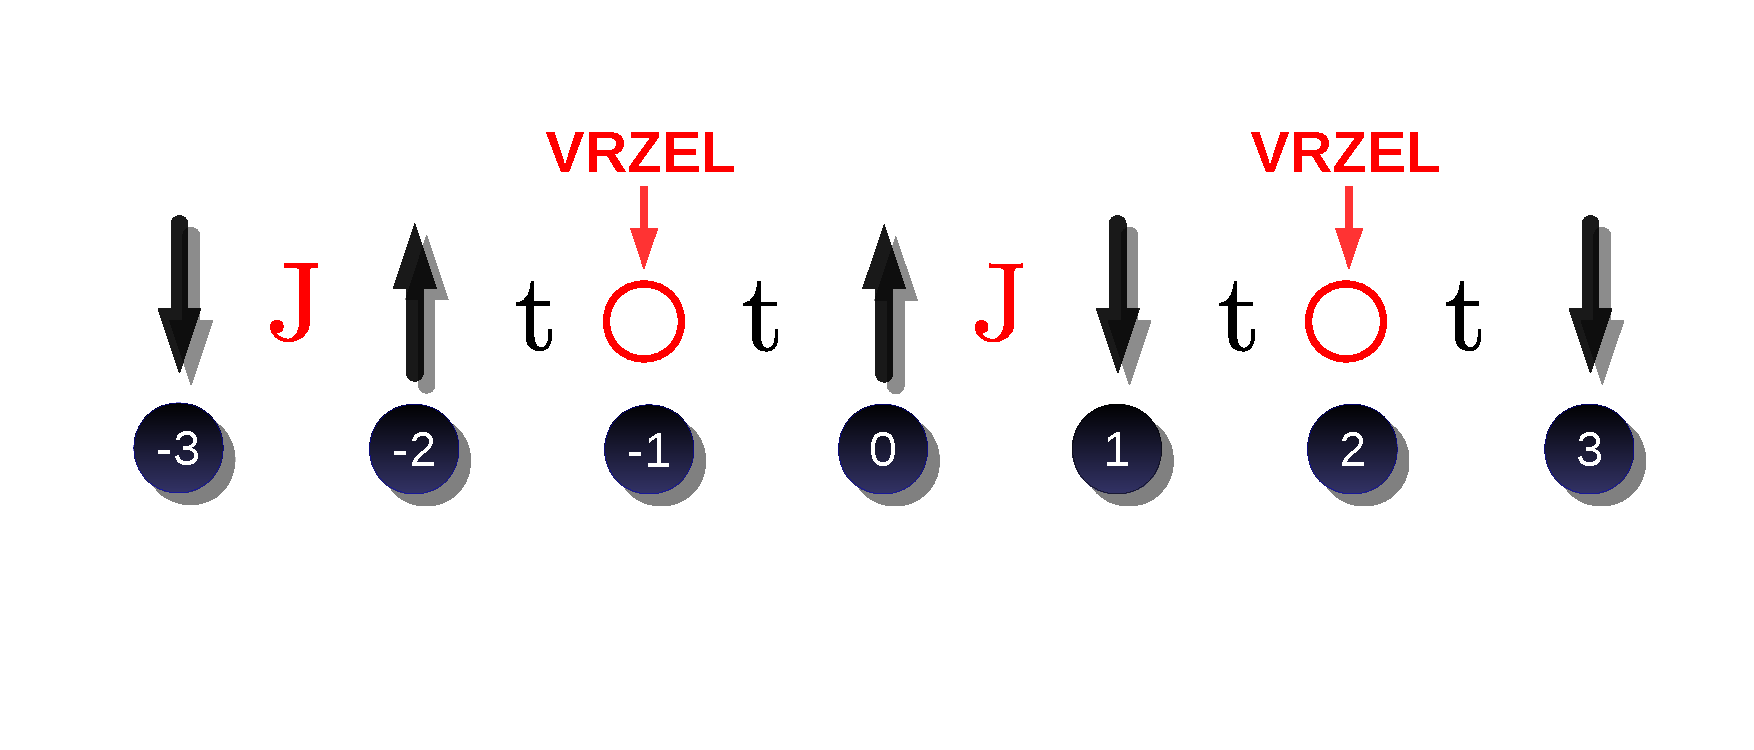
\includegraphics[width=0.7\textwidth]{tJ_scheme.pdf}}
\caption{Oznake: $L$ - št. mest, $N_h$ - št. vrzeli, $N_u$ - število spinov $\uparrow$}
\end{figure} 
\end{minipage}
% \begin{figure}
% \centering{
% 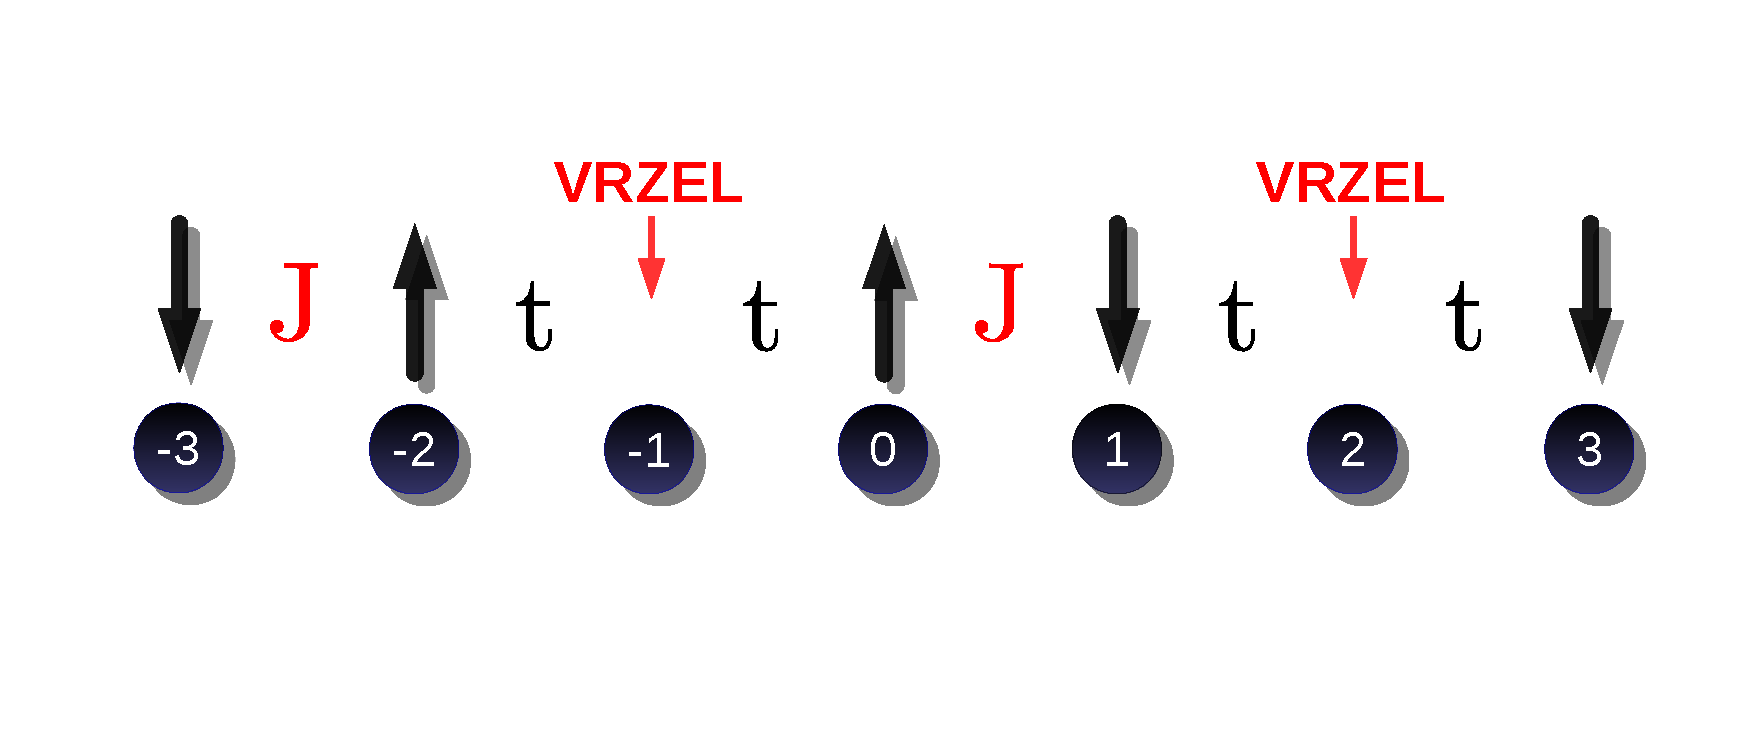
\includegraphics[width=0.5\textwidth]{tJ_scheme_vrzel.pdf}}
% \caption{Oznake: $L$ - št. mest, $N_h$ - št. vrzeli, $N_u$ - število spinov $\uparrow$}
% \end{figure}
\begin{figure}
\centering{
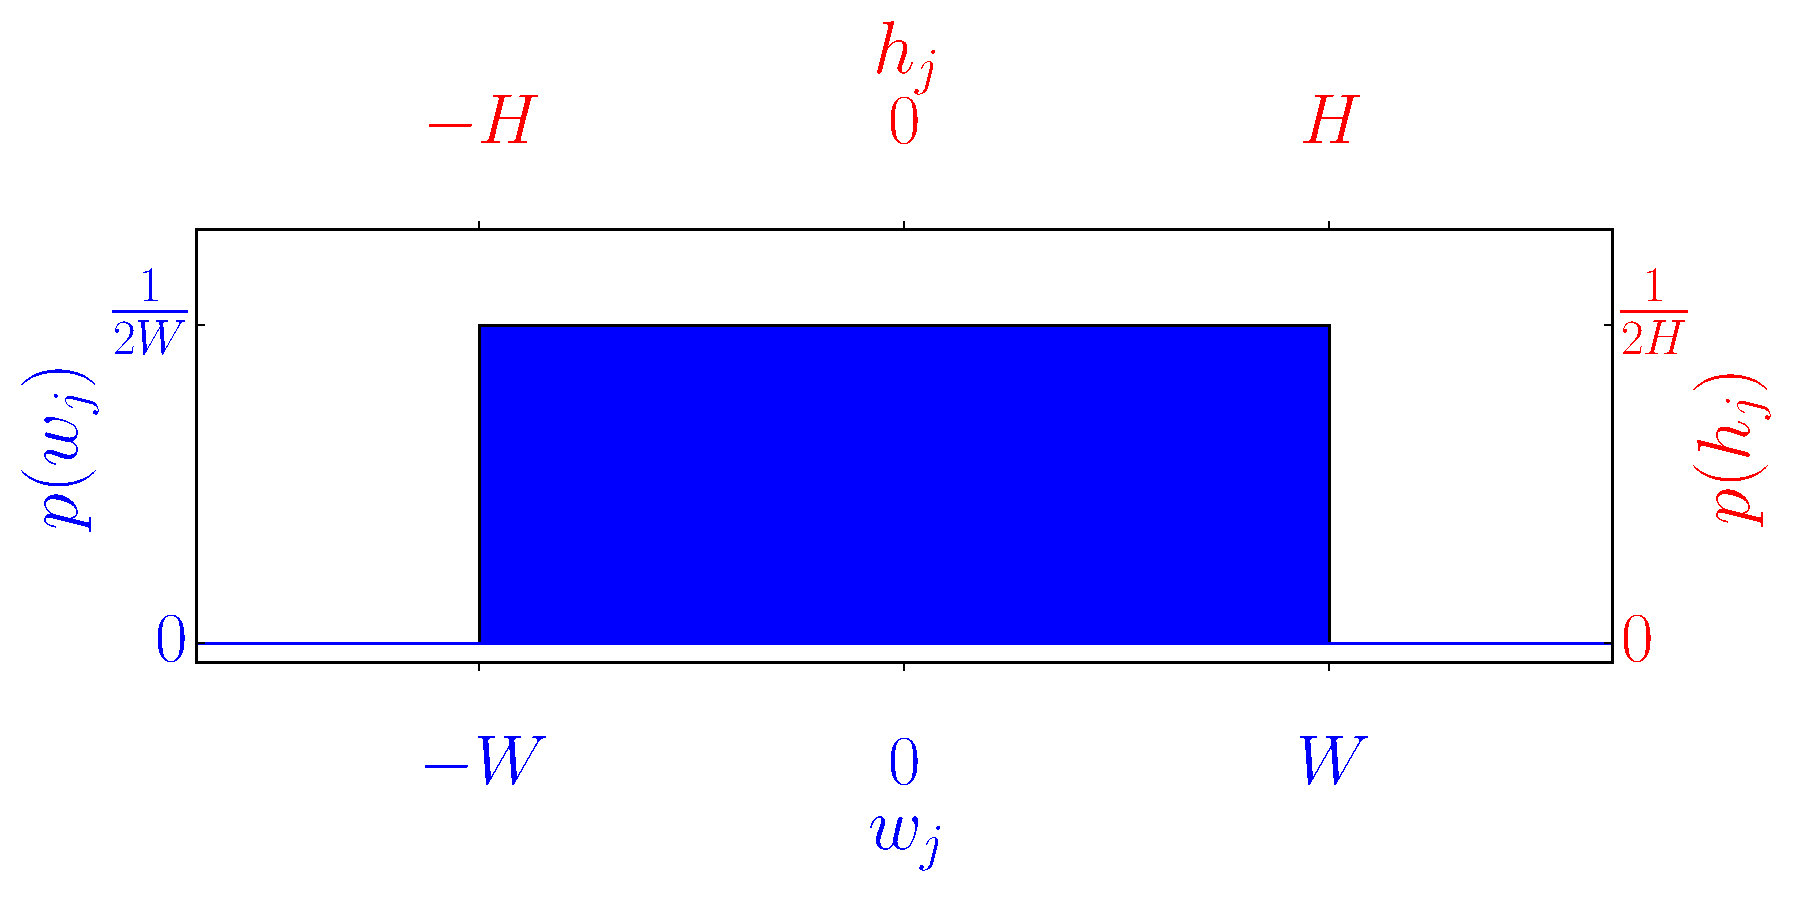
\includegraphics[width=0.5\textwidth]{prob_dist.pdf}}
\caption{Spinski ($W$) in vrzelni ($H$) nered}
\end{figure}
}
\end{frame}

% \begin{frame}{Preučevanje spektralne statistike}
% \only<1>{
% \begin{itemize}
% \item Preučujemo \textbf{porazdelitev razmikov} med sosednjimi nivoji v spektru hamiltonke \vspace{7mm}
% \item Upoštevamo \textbf{teorijo naključnih matrik (RMT):} \vspace{5mm}
% 	\begin{itemize}
% 		\item \textbf{Ergodični} sistemi: spektralna statistika ustreza Gaussovemu ortogonalnemu ansamblu (\textbf{GOE}) \vspace{3mm}
% 		\item \textbf{MBL} sistemi: sosednji nivoji porazdeljeni v skladu s \textbf{Poissonovo} porazdelitvijo, med njimi ni odboja

% 	\end{itemize}\vspace{5mm}
% % \item Further reading:
% % 	\begin{itemize}
% % 		\item Oganesyan, Huse, PRB \textbf{75}, 15511 (2007)
% % 		\item Y.Y. Atas \emph{et. al.}, PRL \textbf{110}, 084101 (2013)
% % 	\end{itemize}
% \end{itemize}}

% % \end{frame}

% % \begin{frame}{Preučevanje spektralne statistike}
% \only<2>{
% Primeri statistik v ergodičnem, vmesnem in MBL režimu
% \begin{figure}
% \centering{
% 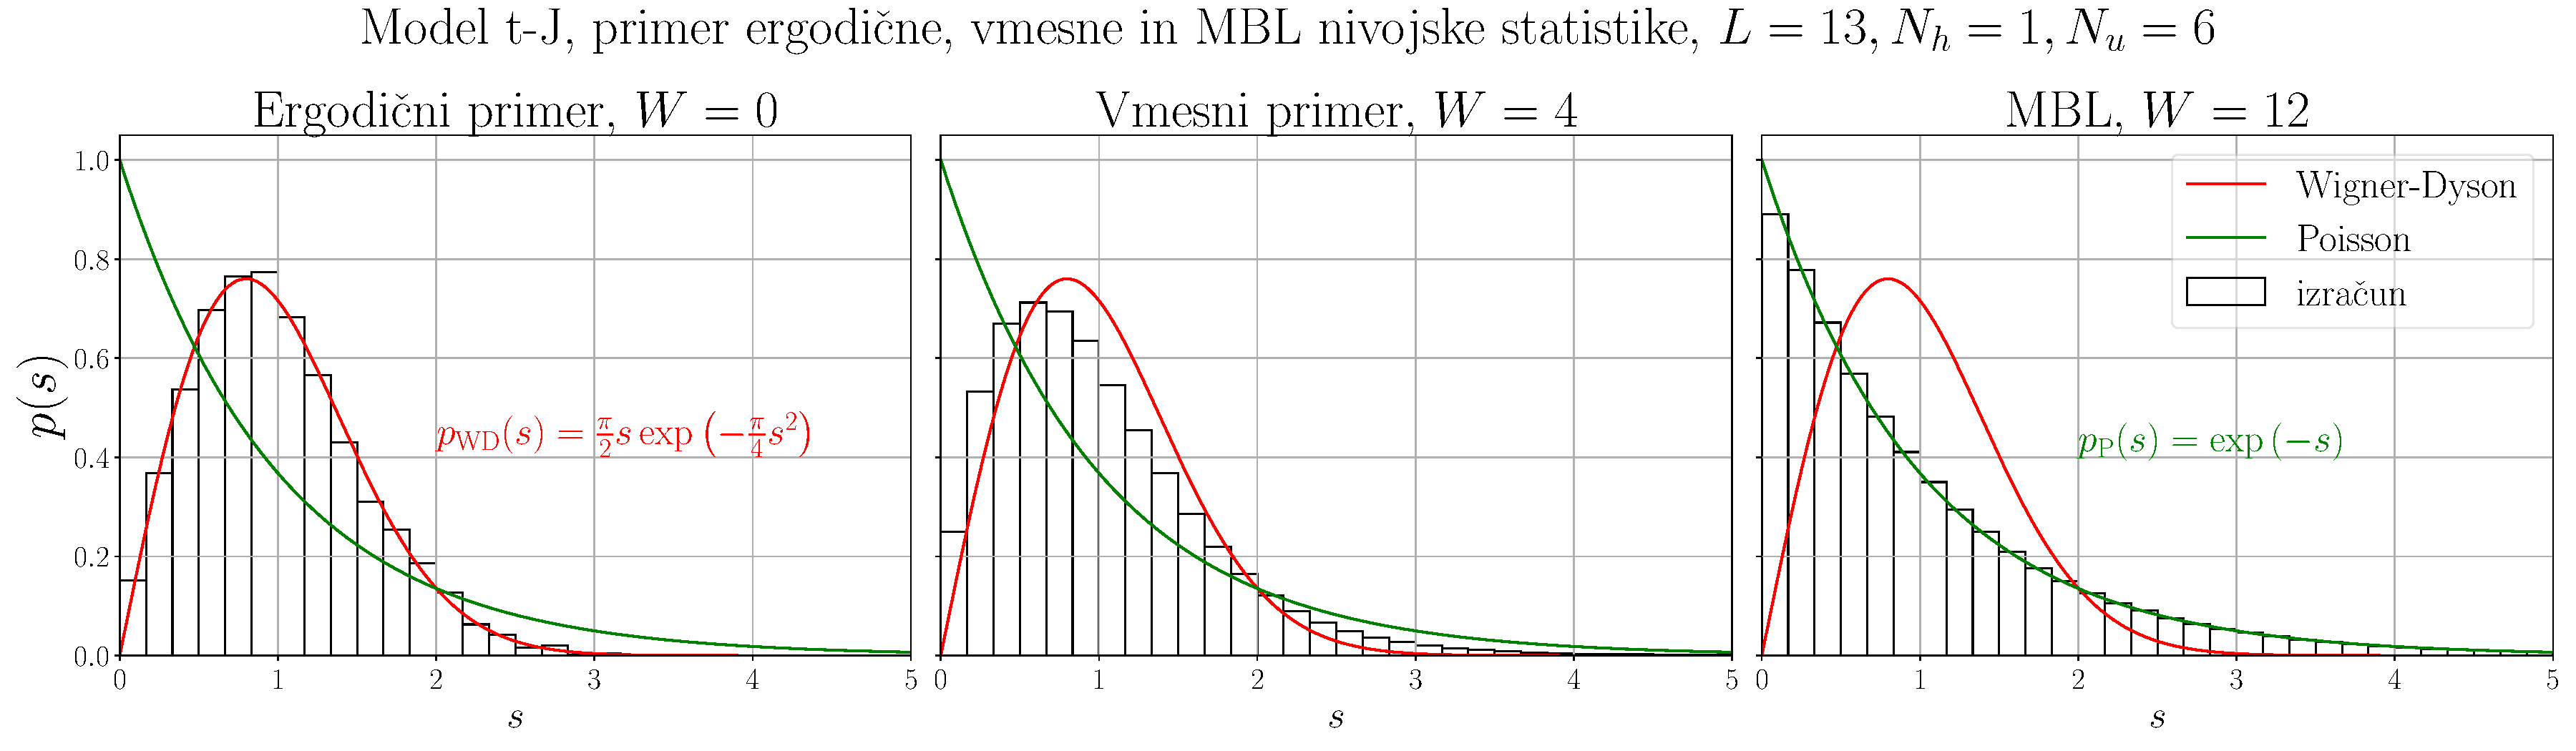
\includegraphics[trim=0 0 0 40,clip,width=1\textwidth]{unfolding_demo_three_slo.pdf}}
% % \caption{$L$ - system size, $N_h$ - number of holes, $N_u$ - number of up spins.}
% \end{figure}
% \begin{minipage}{0.48\textwidth}
% \centering \textbf{GOE:} Wigner-Dysonova porazdelitev
% \end{minipage}\hfill
% \begin{minipage}{0.48\textwidth}
% \centering \textbf{MBL:} Poissonova porazdelitev 
% \end{minipage}}
% \end{frame}


\begin{frame}{Povprečno razmerje razmikov}
\only<1,2>{
\begin{itemize}
\item Analiziramo \textbf{statistične lastnosti} energijskega spektra hamiltonke \vspace{8mm}
\item Upoštevamo \textbf{teorijo naključnih matrik (RMT):} \vspace{7mm}
	\begin{itemize}
		\item \textbf{Ergodični} sistemi: spektralna statistika ustreza Gaussovemu ortogonalnemu ansamblu (\textbf{GOE}) \vspace{3mm}
		\item \textbf{MBL} sistemi: sosednji nivoji porazdeljeni v skladu s \textbf{Poissonovo} porazdelitvijo

	\end{itemize}\vspace{5mm}
\item Upoštevamo korelacije med \textbf{NAJBLIŽJIMI} nivoji v spektru!
\end{itemize}}
\only<2>{
\begin{tikzpicture}[remember picture,overlay]
\node at (current page.center) {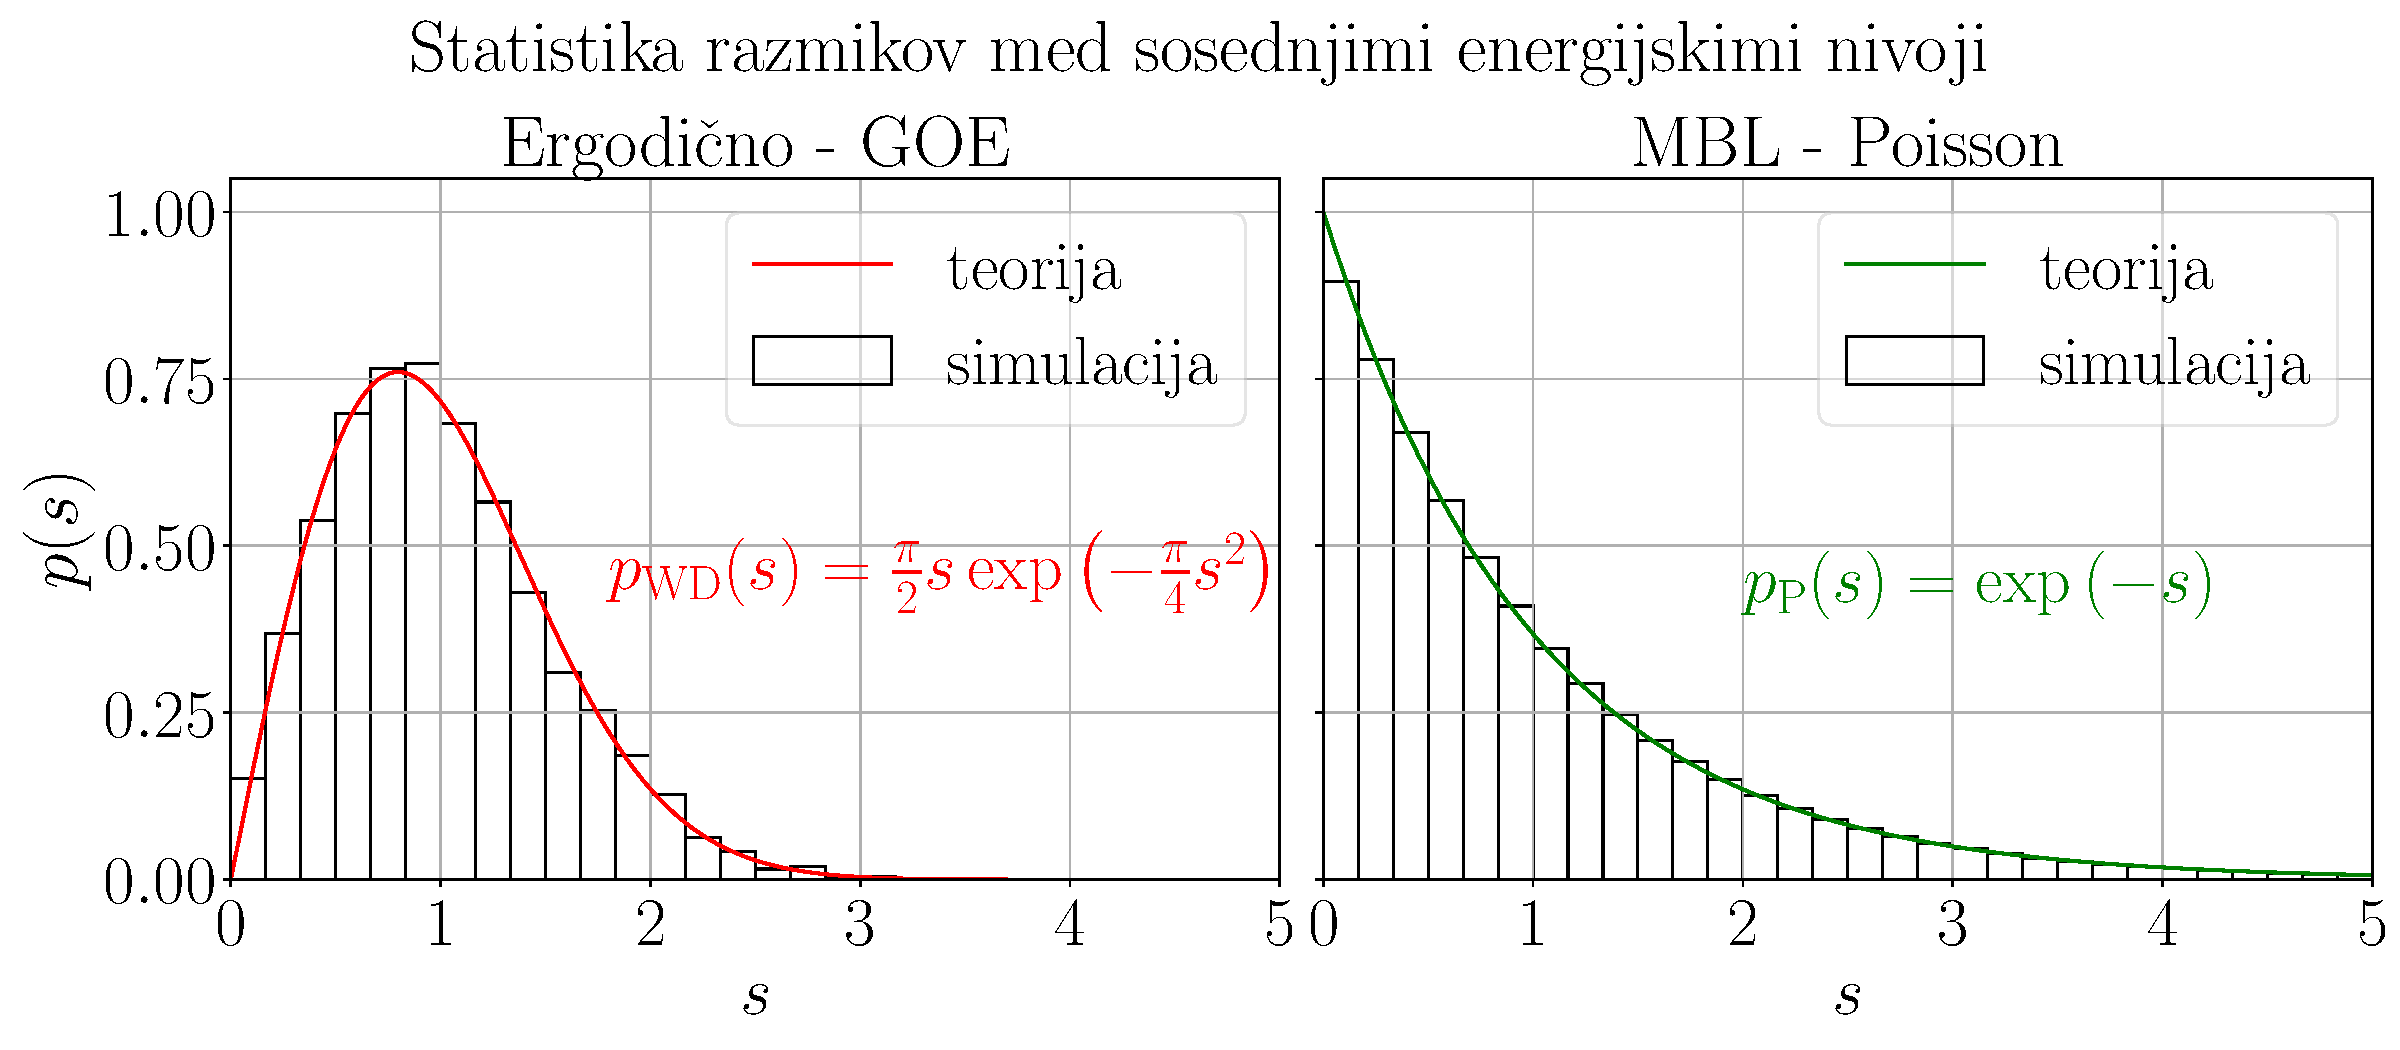
\includegraphics[width=1\textwidth]{unfolding_demo_two_slo.pdf}};
\end{tikzpicture}}

\only<3,4>{
\begin{itemize}
	\onslide<3->{
	\item Razmiki med \textbf{sosednjimi} energijskimi nivoji:$$\delta_n=E_{n+1}-E_n \geq 0$$
	\item Definiramo \textbf{razmerje razmikov}:\vspace{3mm}
	$$0\leq r_n=\min\{\delta_n, \delta_{n-1}\}/\max\{\delta_n, \delta_{n-1}\}\leq 1$$}
	\onslide<4->{
	\item \textbf{KLJUČNO:} limitni povprečni vrednosti $\langle r \rangle$ sta dobro znani: \vspace{5mm} 
	% \begin{itemize}
		$$ \langle r \rangle_\mathrm{GOE}=0.5307, \hspace{5mm} \langle r\rangle_\mathrm{P}=2\ln2 - 1 \approx 0.3863 $$}
		% \item $\langle r \rangle_\mathrm{GOE}=0.5307$ \vspace{3mm}
		% \item $\langle r\rangle_\mathrm{P}=2\ln2 - 1 \approx 0.386$
	% \end{itemize}
\end{itemize}}

\end{frame}

\begin{frame}{Rezultati}
\only<1>{
	\textbf{VPRAŠANJE:}\vspace{10mm}
	
	\begin{itemize}
		\centering{\item \textbf{Nastopi MBL za oba tipa nereda?}\vspace{10mm}}
		% \item \textbf{Kakšna je vloga dopiranja?}	
	\end{itemize}
}
% \only<2,3>{
% 	Dopiranje z eno vrzeljo, $N_h=1$:
% 	\begin{figure}
% 	\centering{
% 	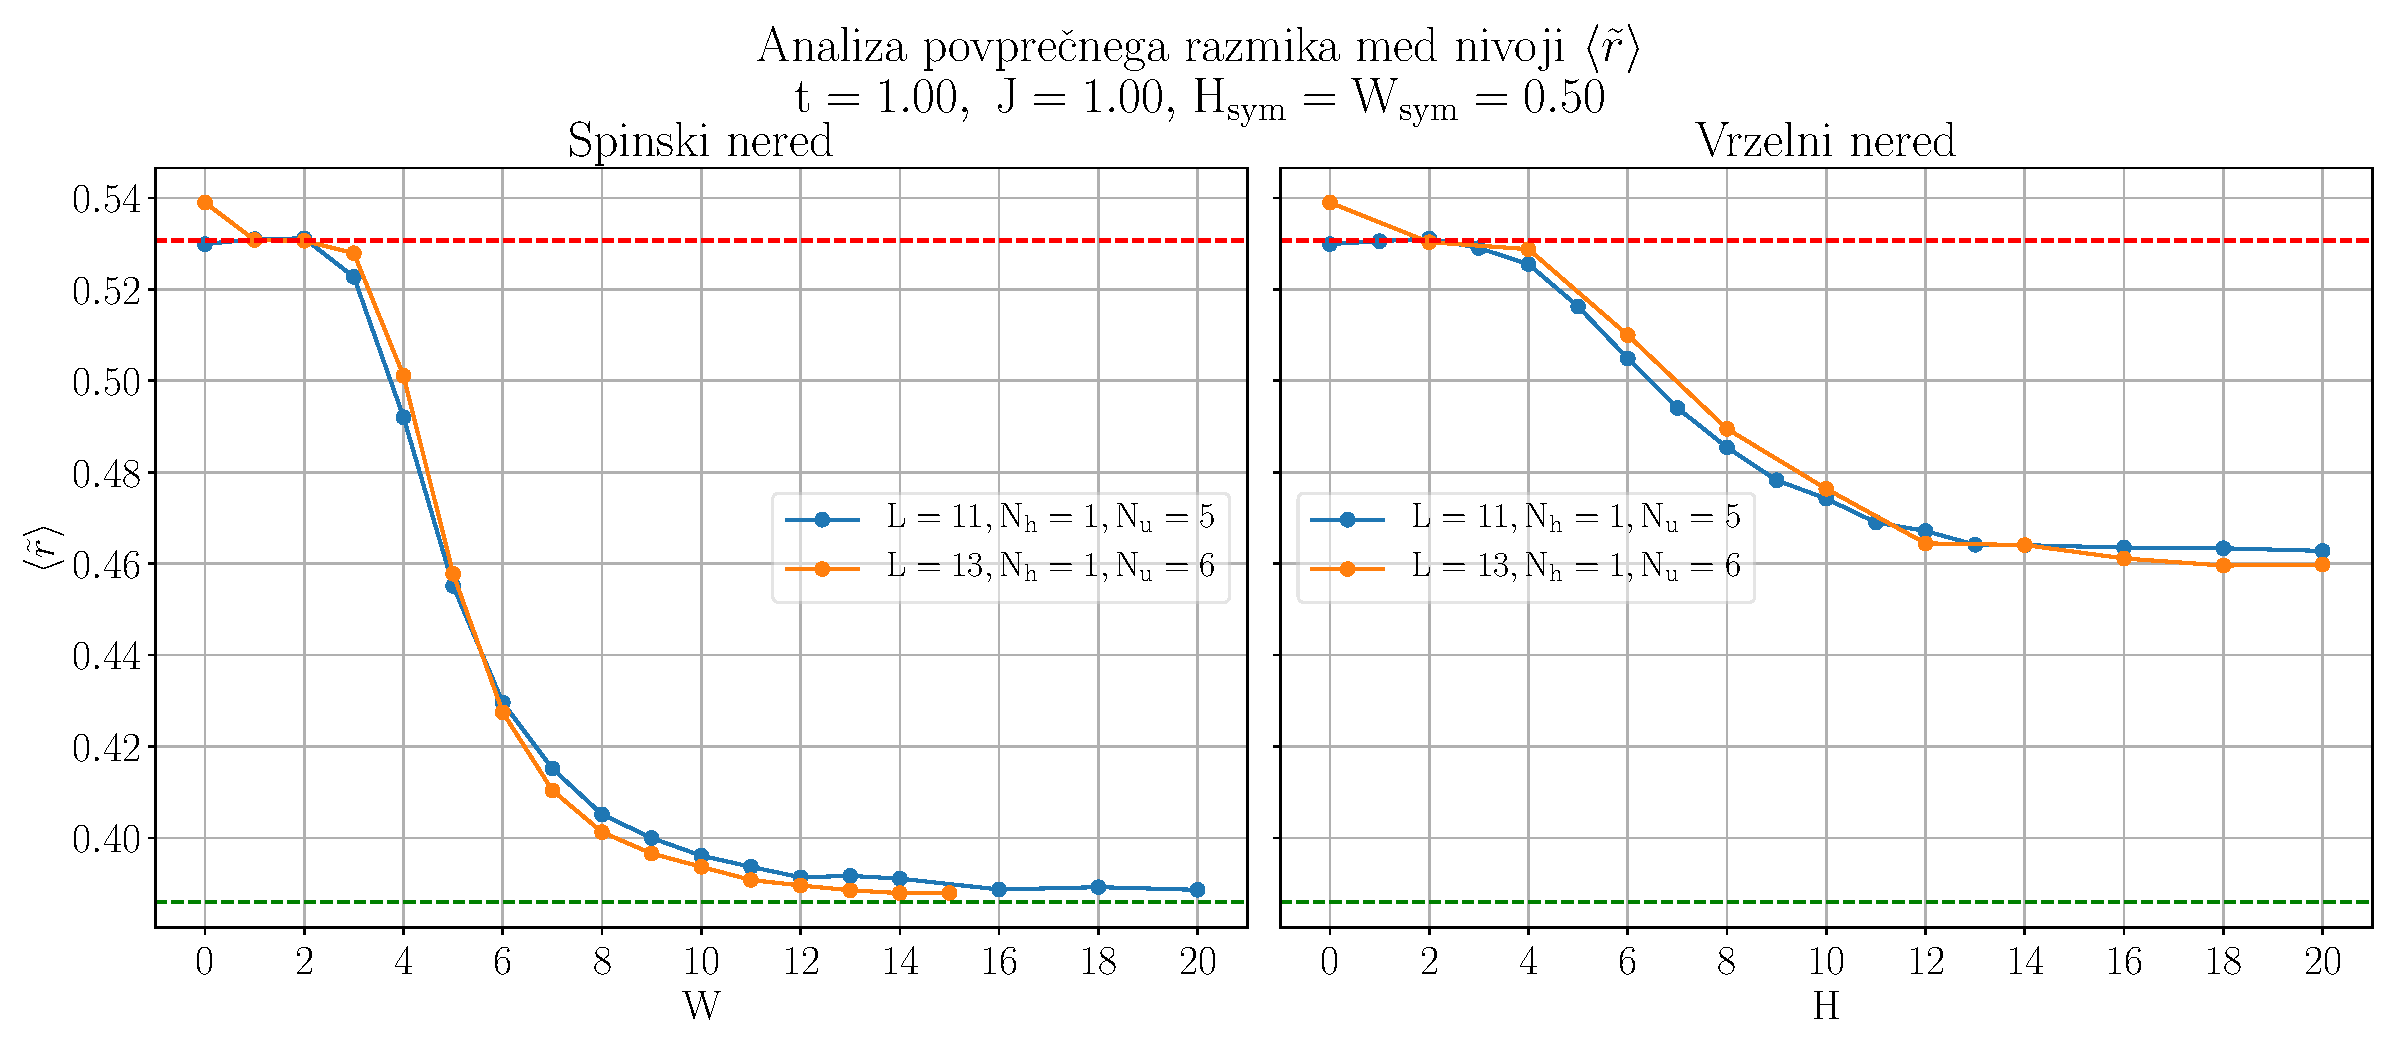
\includegraphics[trim=0 0 0 58,clip,width=1\textwidth]{double_plot_disorder_sym_break_13_1_6_slo.pdf}}
% 	\end{figure}
% 	\onslide<3->{
% 	\textbf{VRZELNI NERED: ni MBL}}}
\only<2,3>{
	Tretjinsko dopiranje, $N_h=L/3$:
	\begin{figure}
	\centering{
	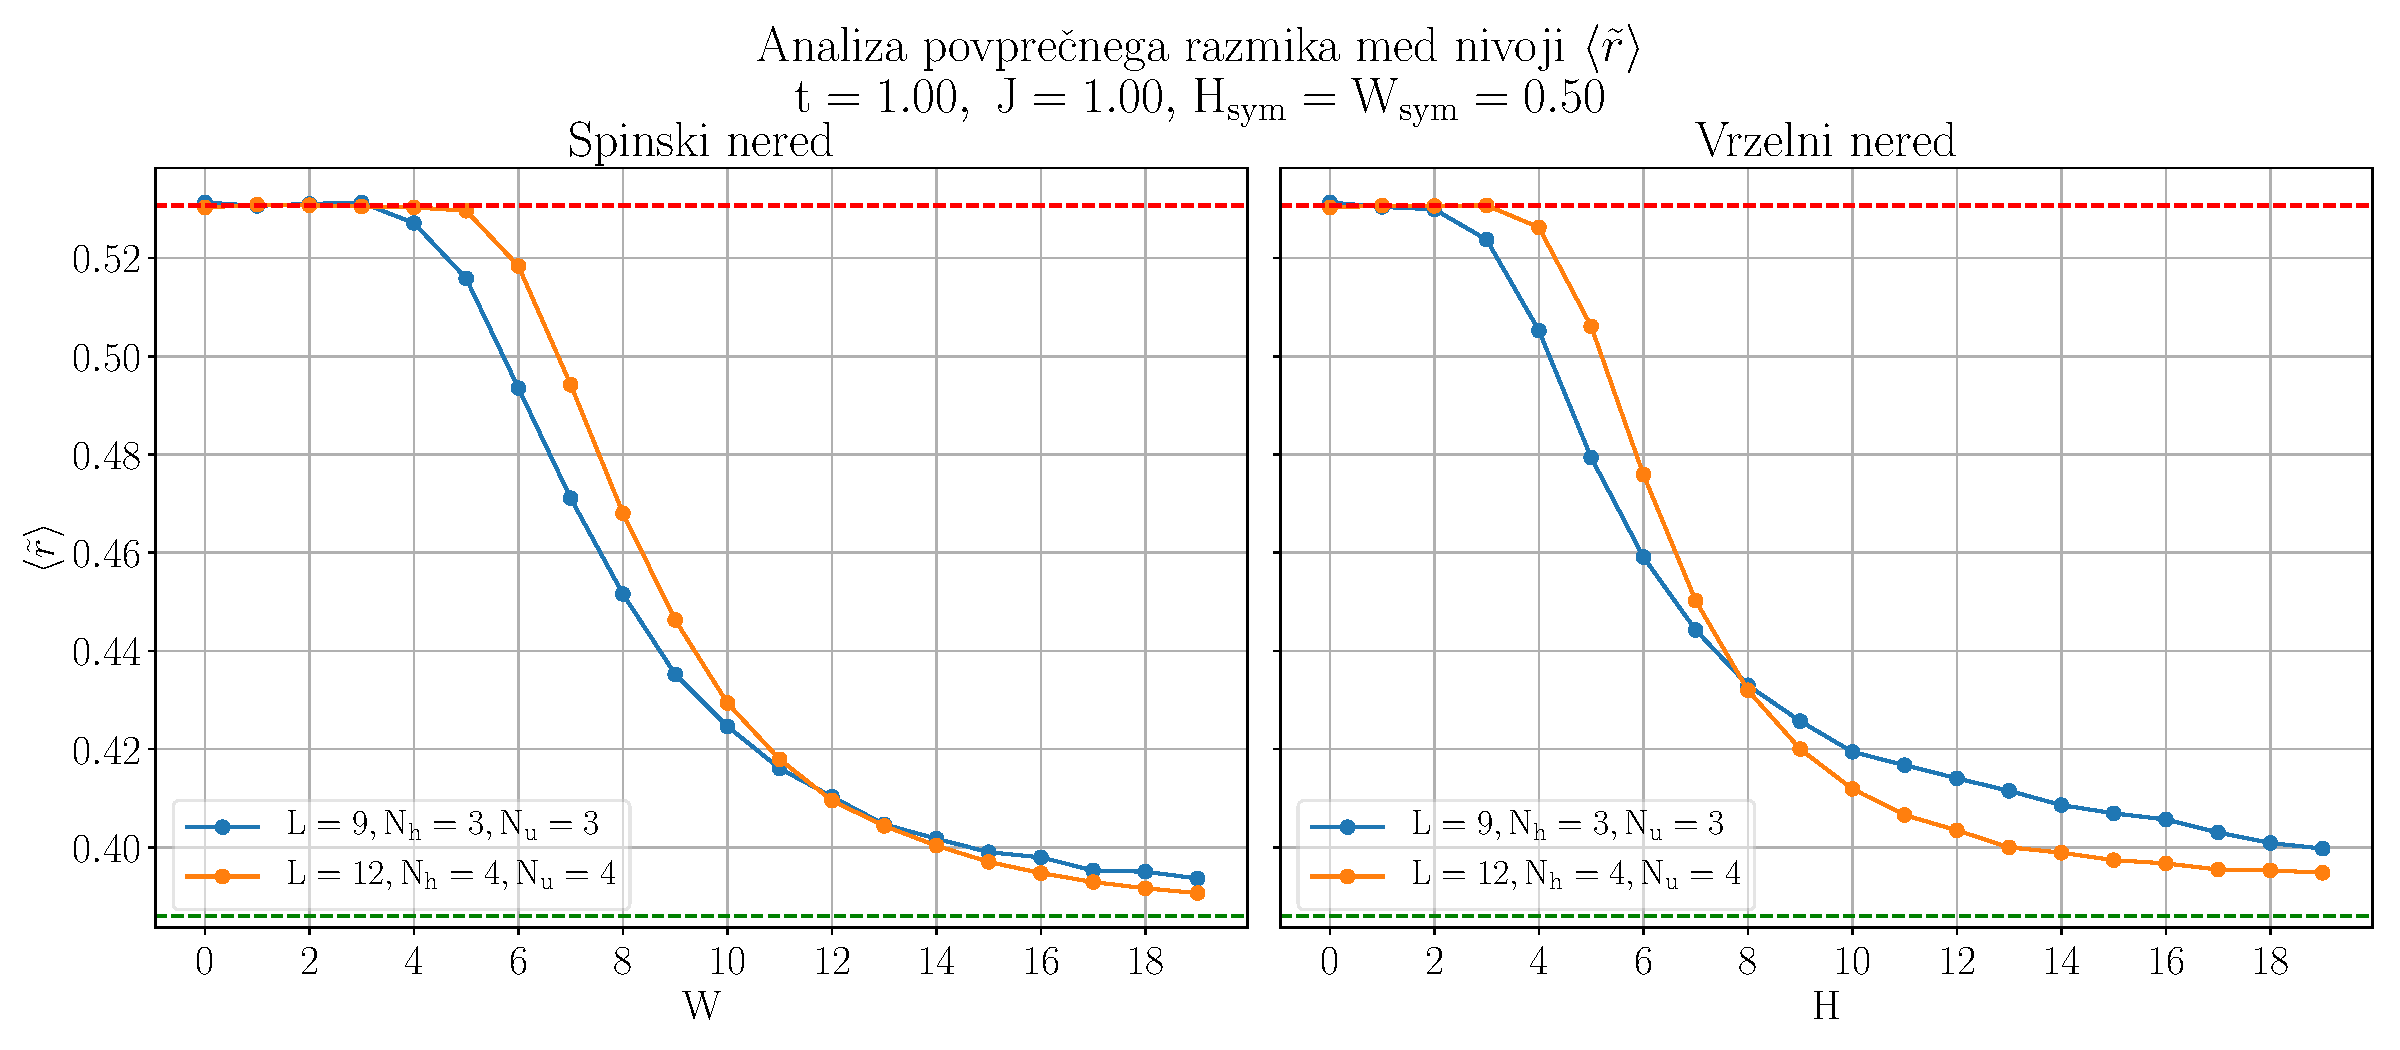
\includegraphics[trim=0 0 0 58,clip,width=1\textwidth]{double_plot_disorder_sym_break_12_4_4_slo.pdf}}
	\end{figure}
	\onslide<3->{
	\textbf{MBL za oba tipa nereda}}
}	

\only<4>{
	Oba tipa nereda hkrati\\
	\begin{figure}
	\centering{
	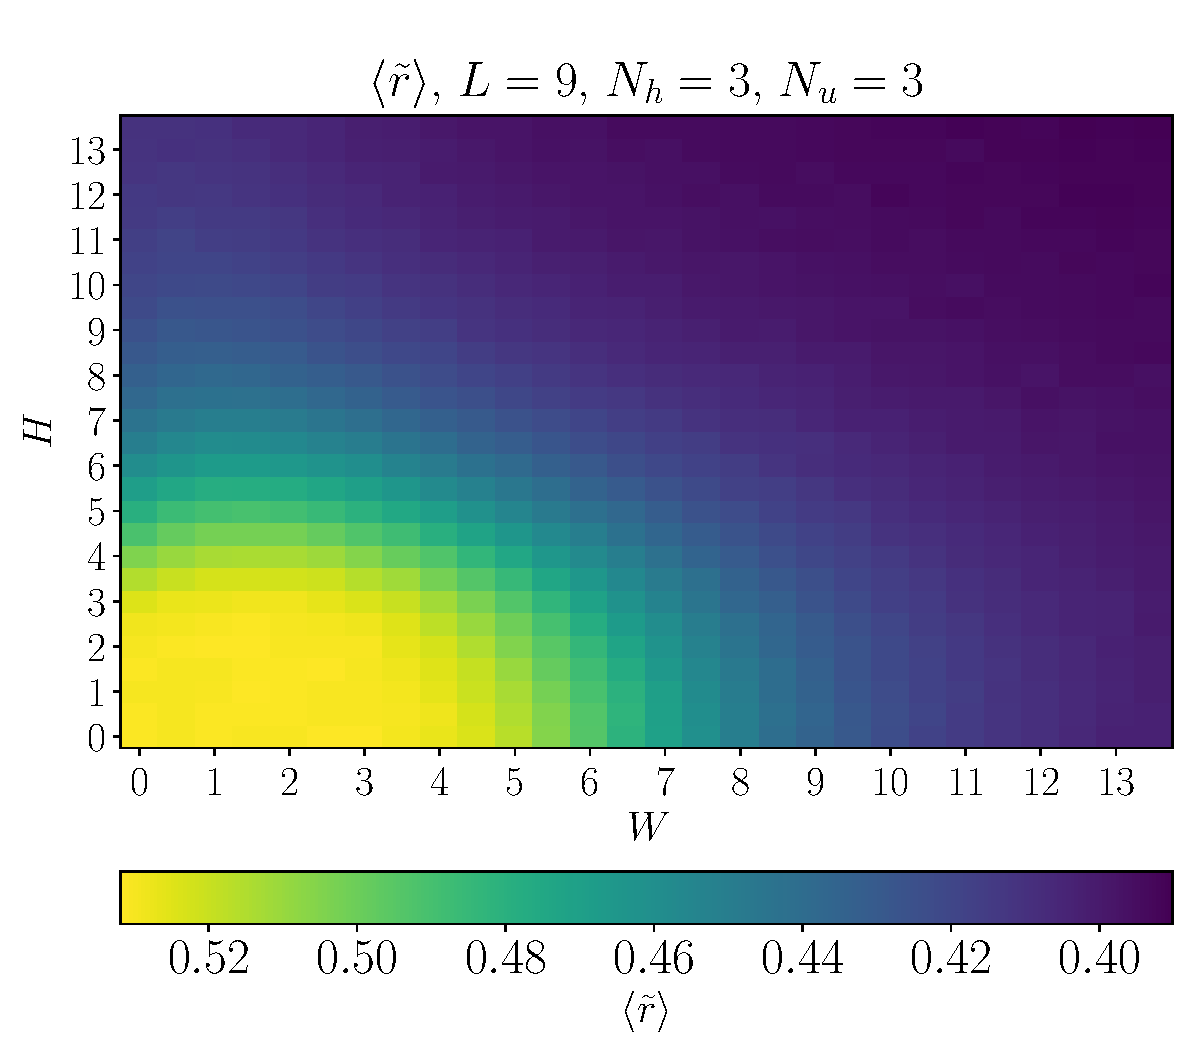
\includegraphics[width=0.6\textwidth]{r_density_9_3_3.pdf}}
	\caption{\textbf{Rumena} $\rightarrow$ ergodično \hspace{5mm} \textbf{Modra} $\rightarrow$ MBL}
	\end{figure}
	% \begin{minipage}[c]{0.48\textwidth}
	% \begin{figure}
	% \centering{
	% 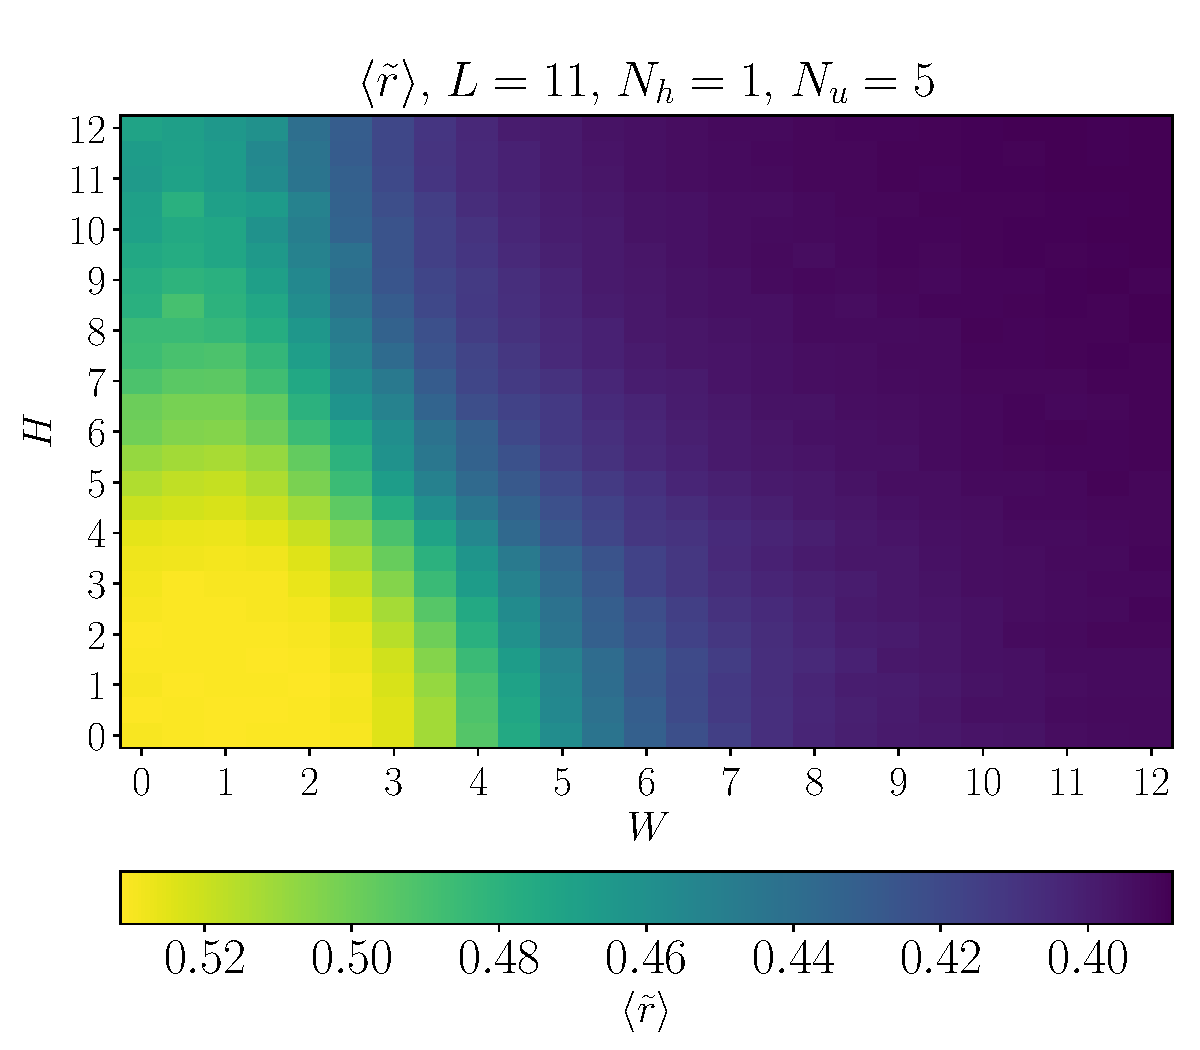
\includegraphics[width=1\textwidth]{r_density_11_1_5.pdf}}
	% \caption{Ena vrzel.}
	% \end{figure}
	% \end{minipage}\hfill
	% \begin{minipage}[c]{0.48\textwidth}
	% \begin{figure}
	% \centering{
	% 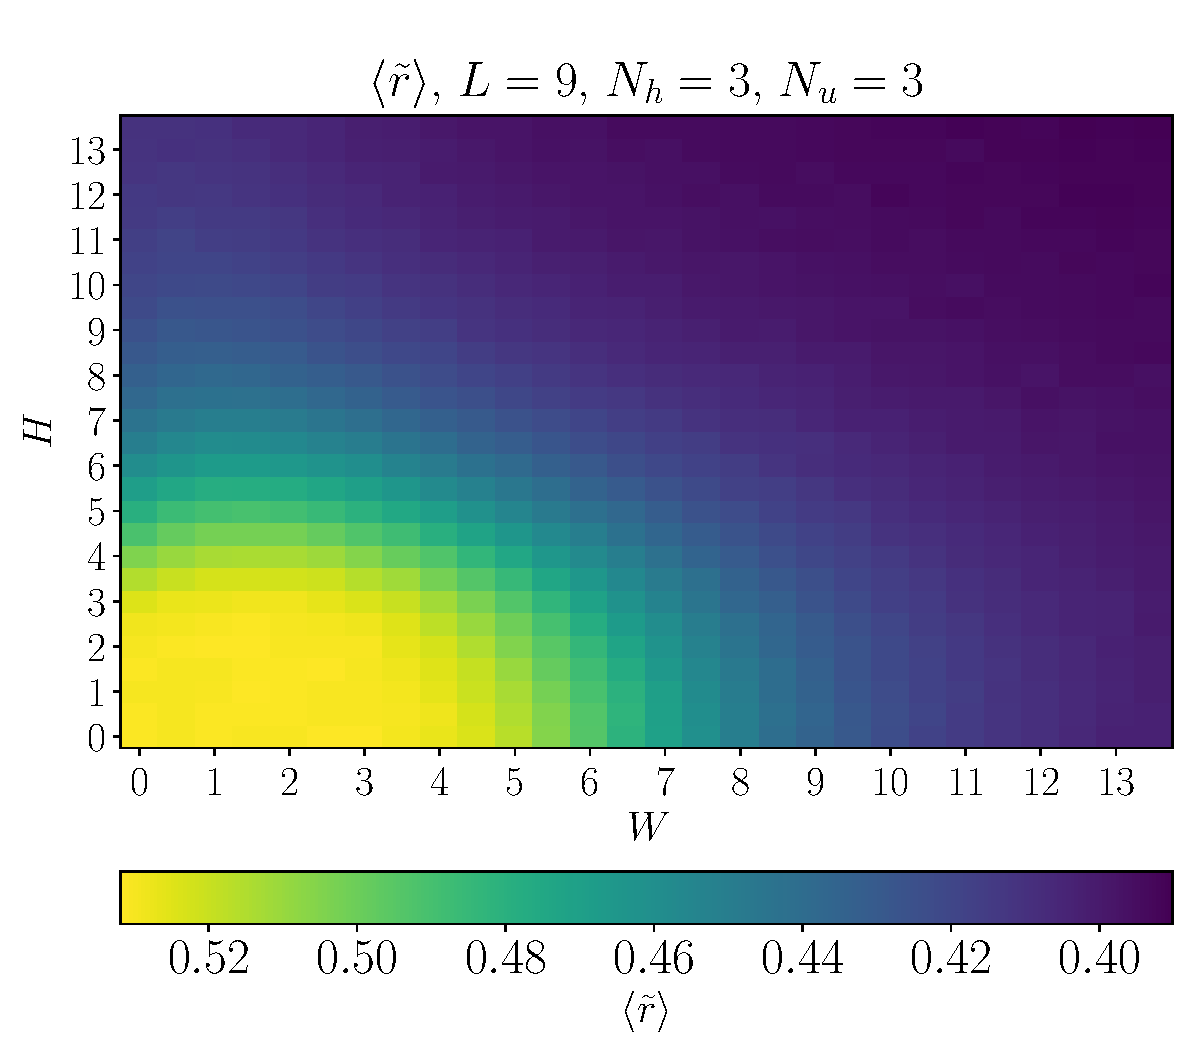
\includegraphics[width=1\textwidth]{r_density_9_3_3.pdf}}
	% \caption{Tretjinsko dopiranje.}
	% \end{figure}
	% \end{minipage}
}



\end{frame}{}

\begin{frame}{Spektralni oblikovni faktor (SFF)}
\only<1>{
\begin{alertblock}{\centering{Definicija}}
$$
K(\tau)\coloneqq  \left\langle \frac{1}{N}\sum\limits_{i,j}^N \mathrm{e}^{-\iu \left(E_i - E_j\right) \tau}\right\rangle
$$
\end{alertblock}
\begin{alertblock}{\centering{Povezani spektralni oblikovni faktor}}
$$
K_\mathrm{c}(\tau)\coloneqq  K(\tau) - \left|\left\langle \frac{1}{\sqrt{N}} \sum\limits_i \mathrm{e}^{-\iu E_i \tau}\right\rangle\right|^2
$$
\end{alertblock}\vspace{10mm}
Upoštevamo korelacije med \textbf{VSEMI} energijskimi nivoji v spektru!

}
\only<2,3>{
\begin{alertblock}{\centering{$K(\tau)$ v ergodičnem sistemu}}
\begin{equation*}\label{eq:ramp}
K_\mathrm{GOE}(\tau)=
\begin{cases}
2\tau - \tau \log\left(1 + 2\tau\right), \hspace{5mm} \tau \leq 1, \\
2 - \tau \log\left(\frac{2\tau + 1}{2\tau - 1}\right),\hspace{5mm} \tau >1.
\end{cases}
\end{equation*} 
\end{alertblock}}
\only<2>{\vspace{10mm}
\begin{alertblock}{\centering{$K(\tau)$ v MBL (in integrabilnih) sistemih}}
\begin{equation*}\label{eq:ramp}
K_\mathrm{P}(\tau)=1
\end{equation*} 
\end{alertblock}
}
\only<3>{
\begin{figure}[H]
\centering{
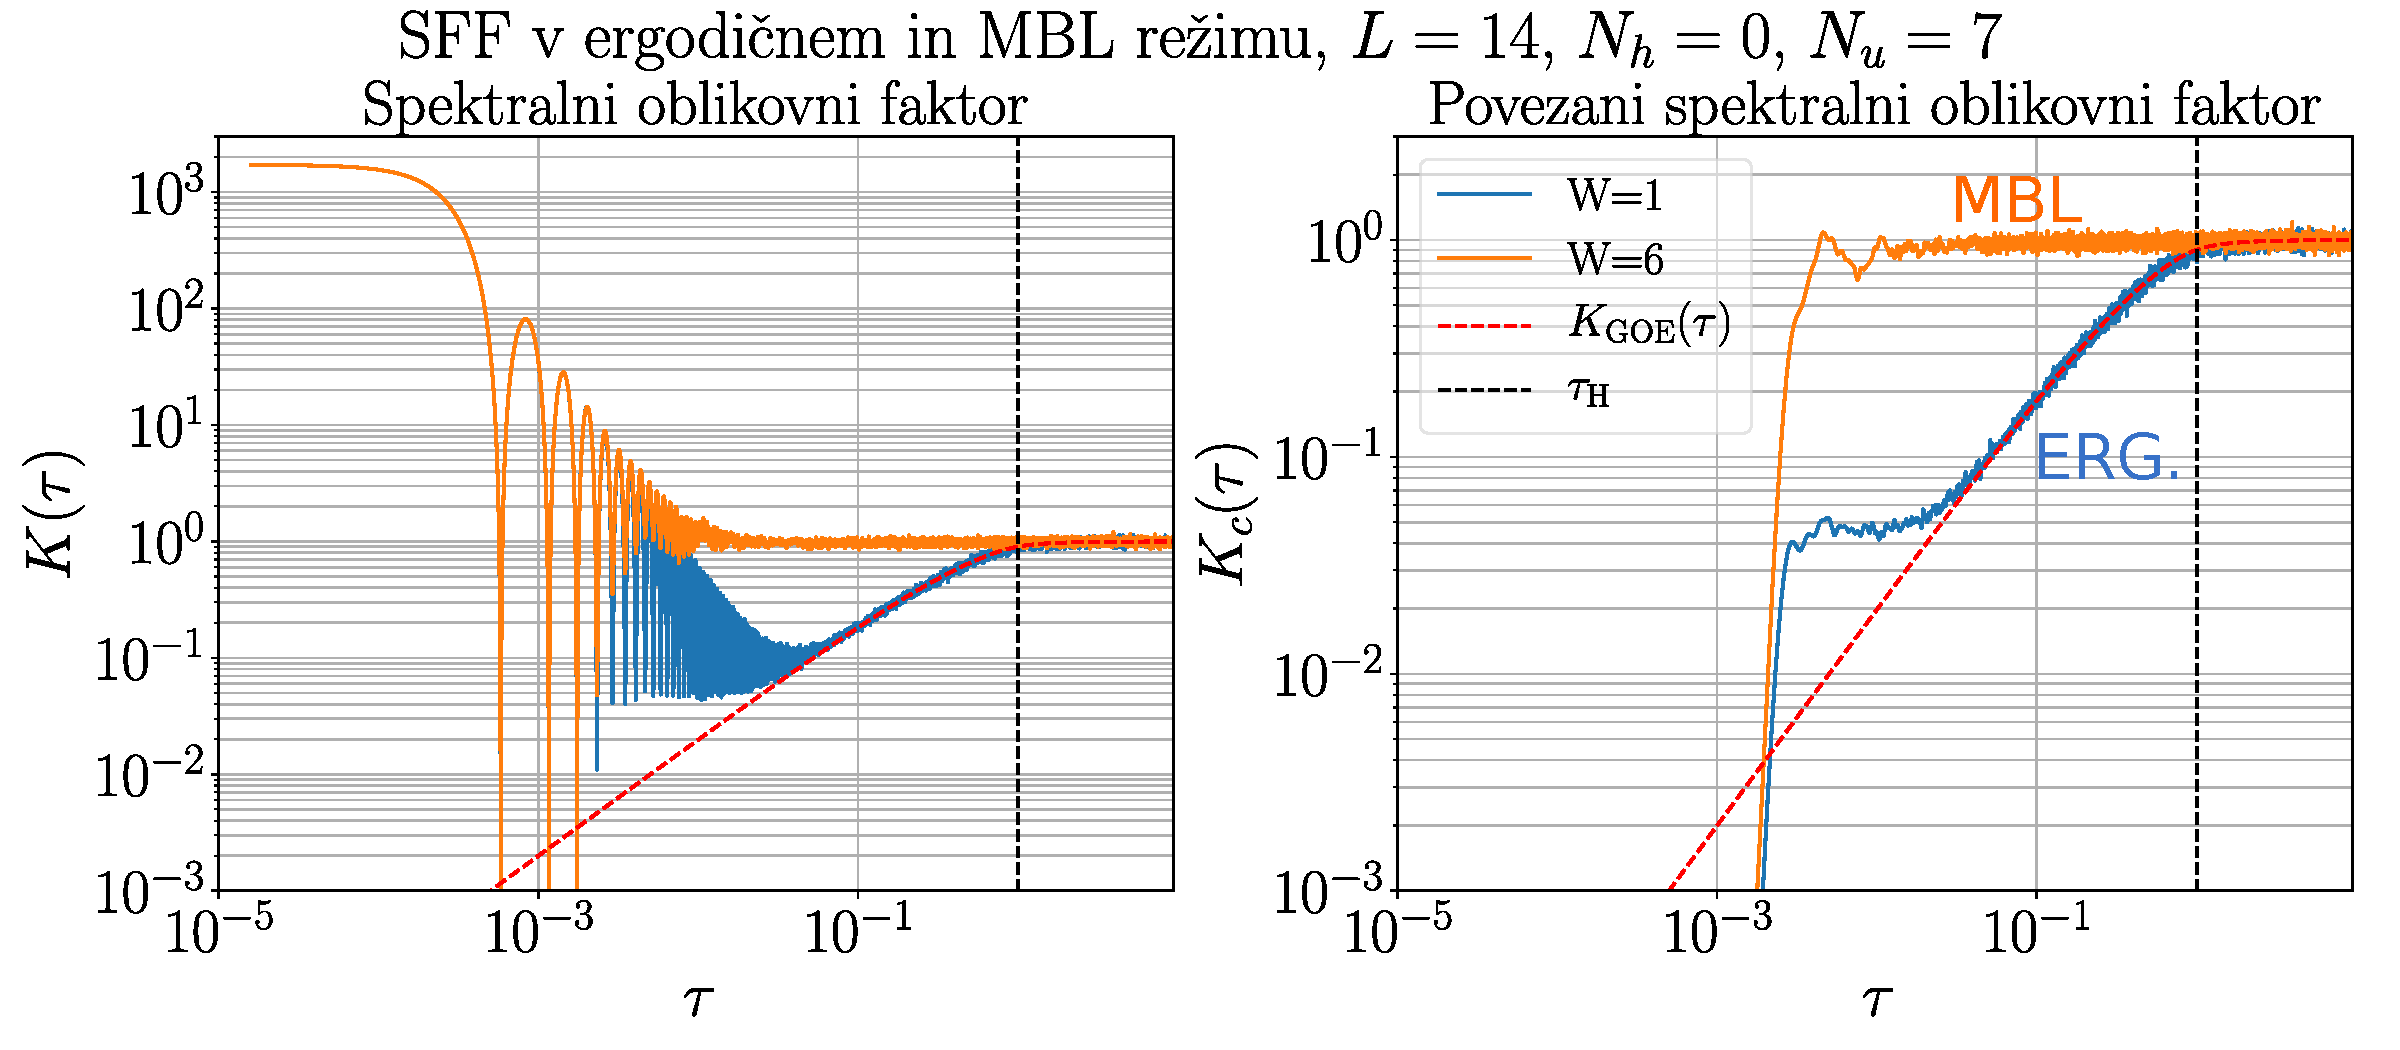
\includegraphics[width=1\textwidth]{scheme_sff_disorder_14_0_7.pdf}}
\caption{}
% \label{fig:scheme_sff_disorder_14_0_7}
\end{figure}  	
}
\end{frame}
\begin{frame}{SFF - rezultati}
% \only<1,2>{
% Ena vrzel - $L=11, N_h=1, N_u=5$\\\vspace{7mm}
% \begin{minipage}[c]{0.48\textwidth}
% \begin{figure}[H]
% \centering{
% 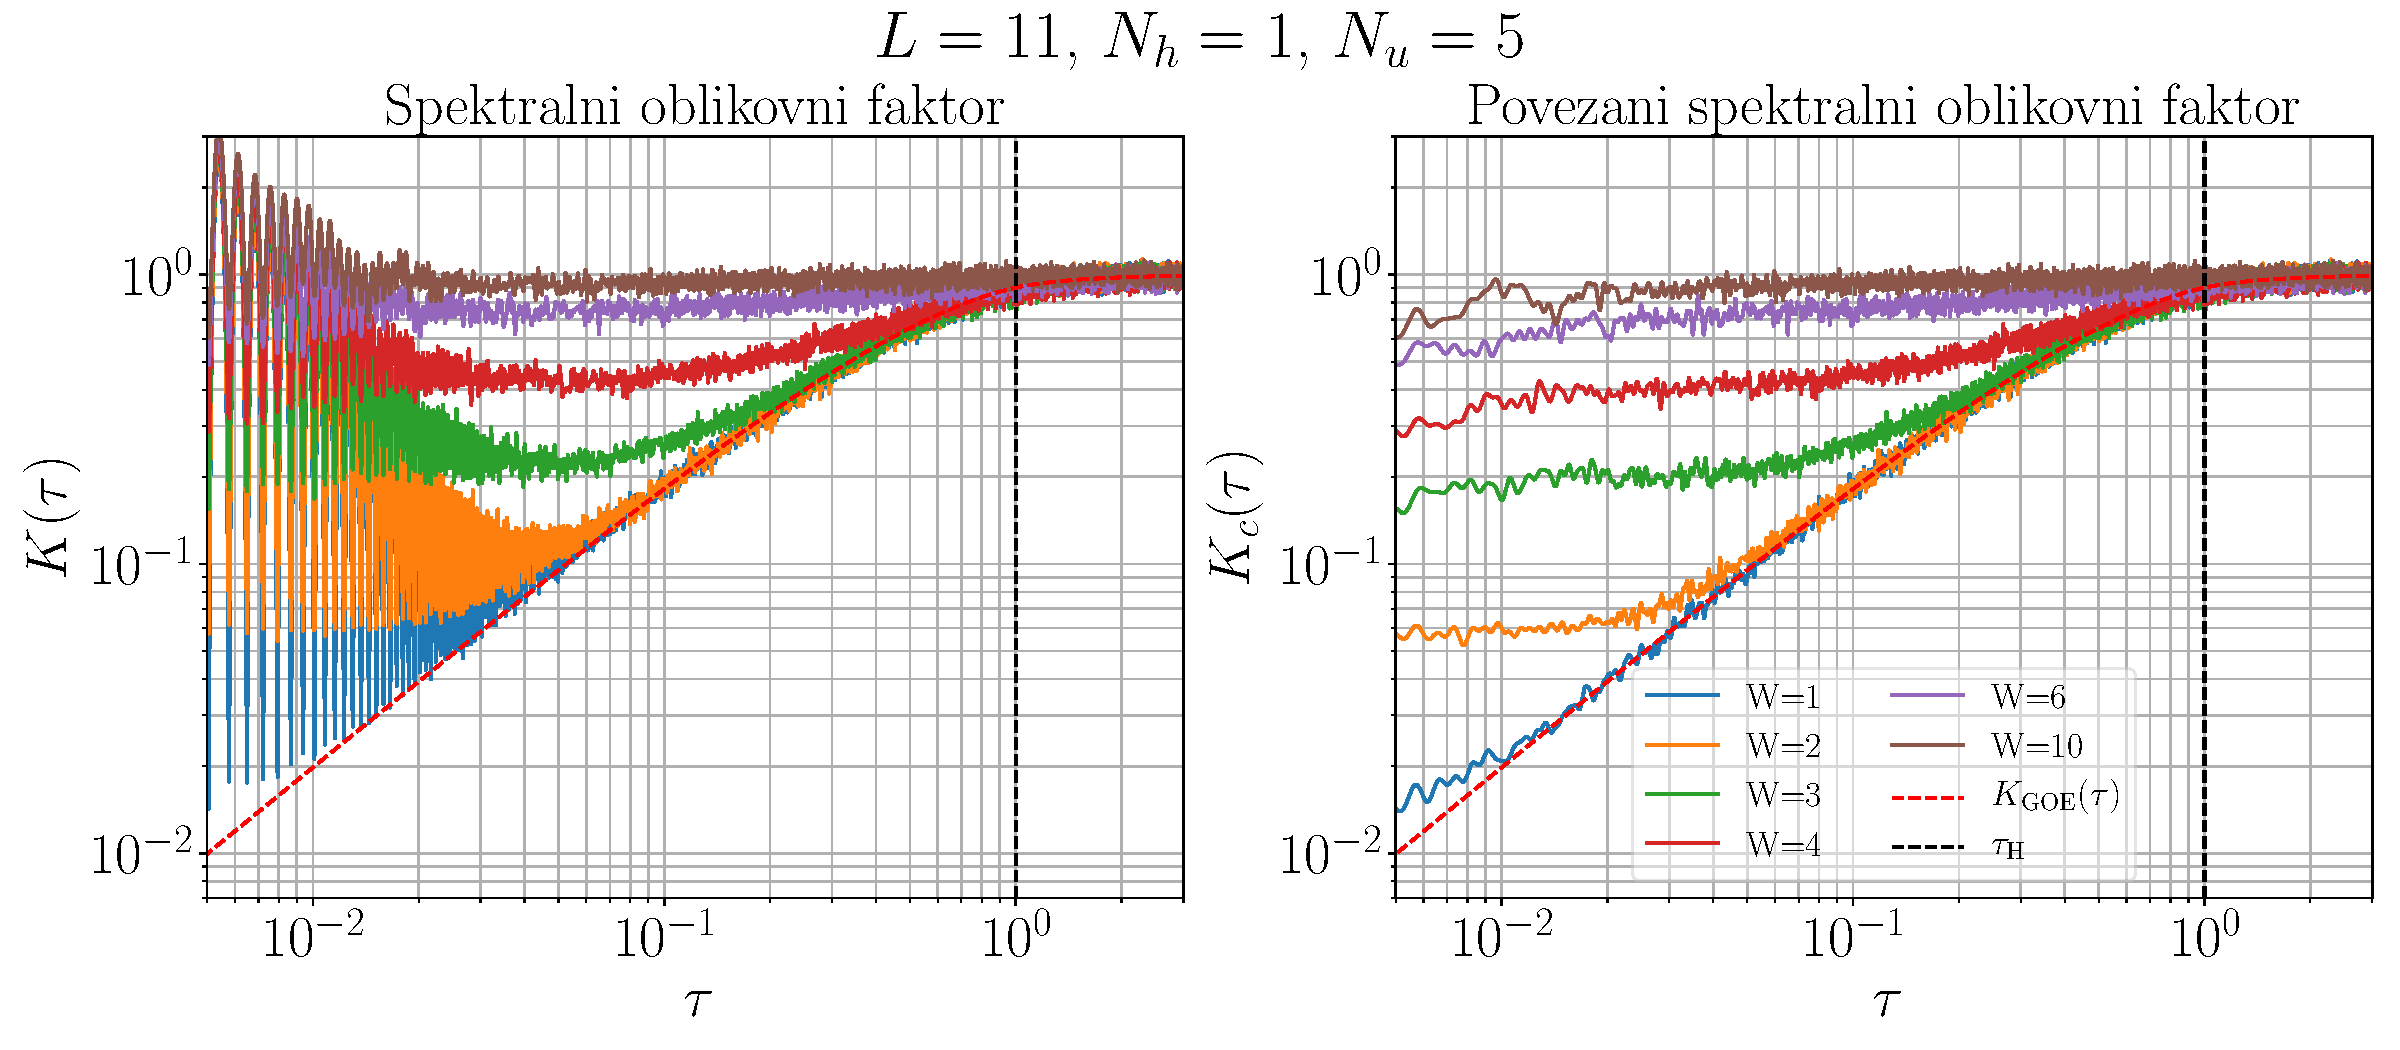
\includegraphics[trim=570 0 0 33,clip,width=1\textwidth]{W_sweep_sff_disorder_11_1_5.pdf}}
% \caption{Spinski nered.}
% % \label{fig:scheme_sff_disorder_14_0_7}
% \end{figure} 
% \end{minipage}\hfill
% \begin{minipage}[c]{0.48\textwidth}
% \begin{figure}[H]
% \centering{
% 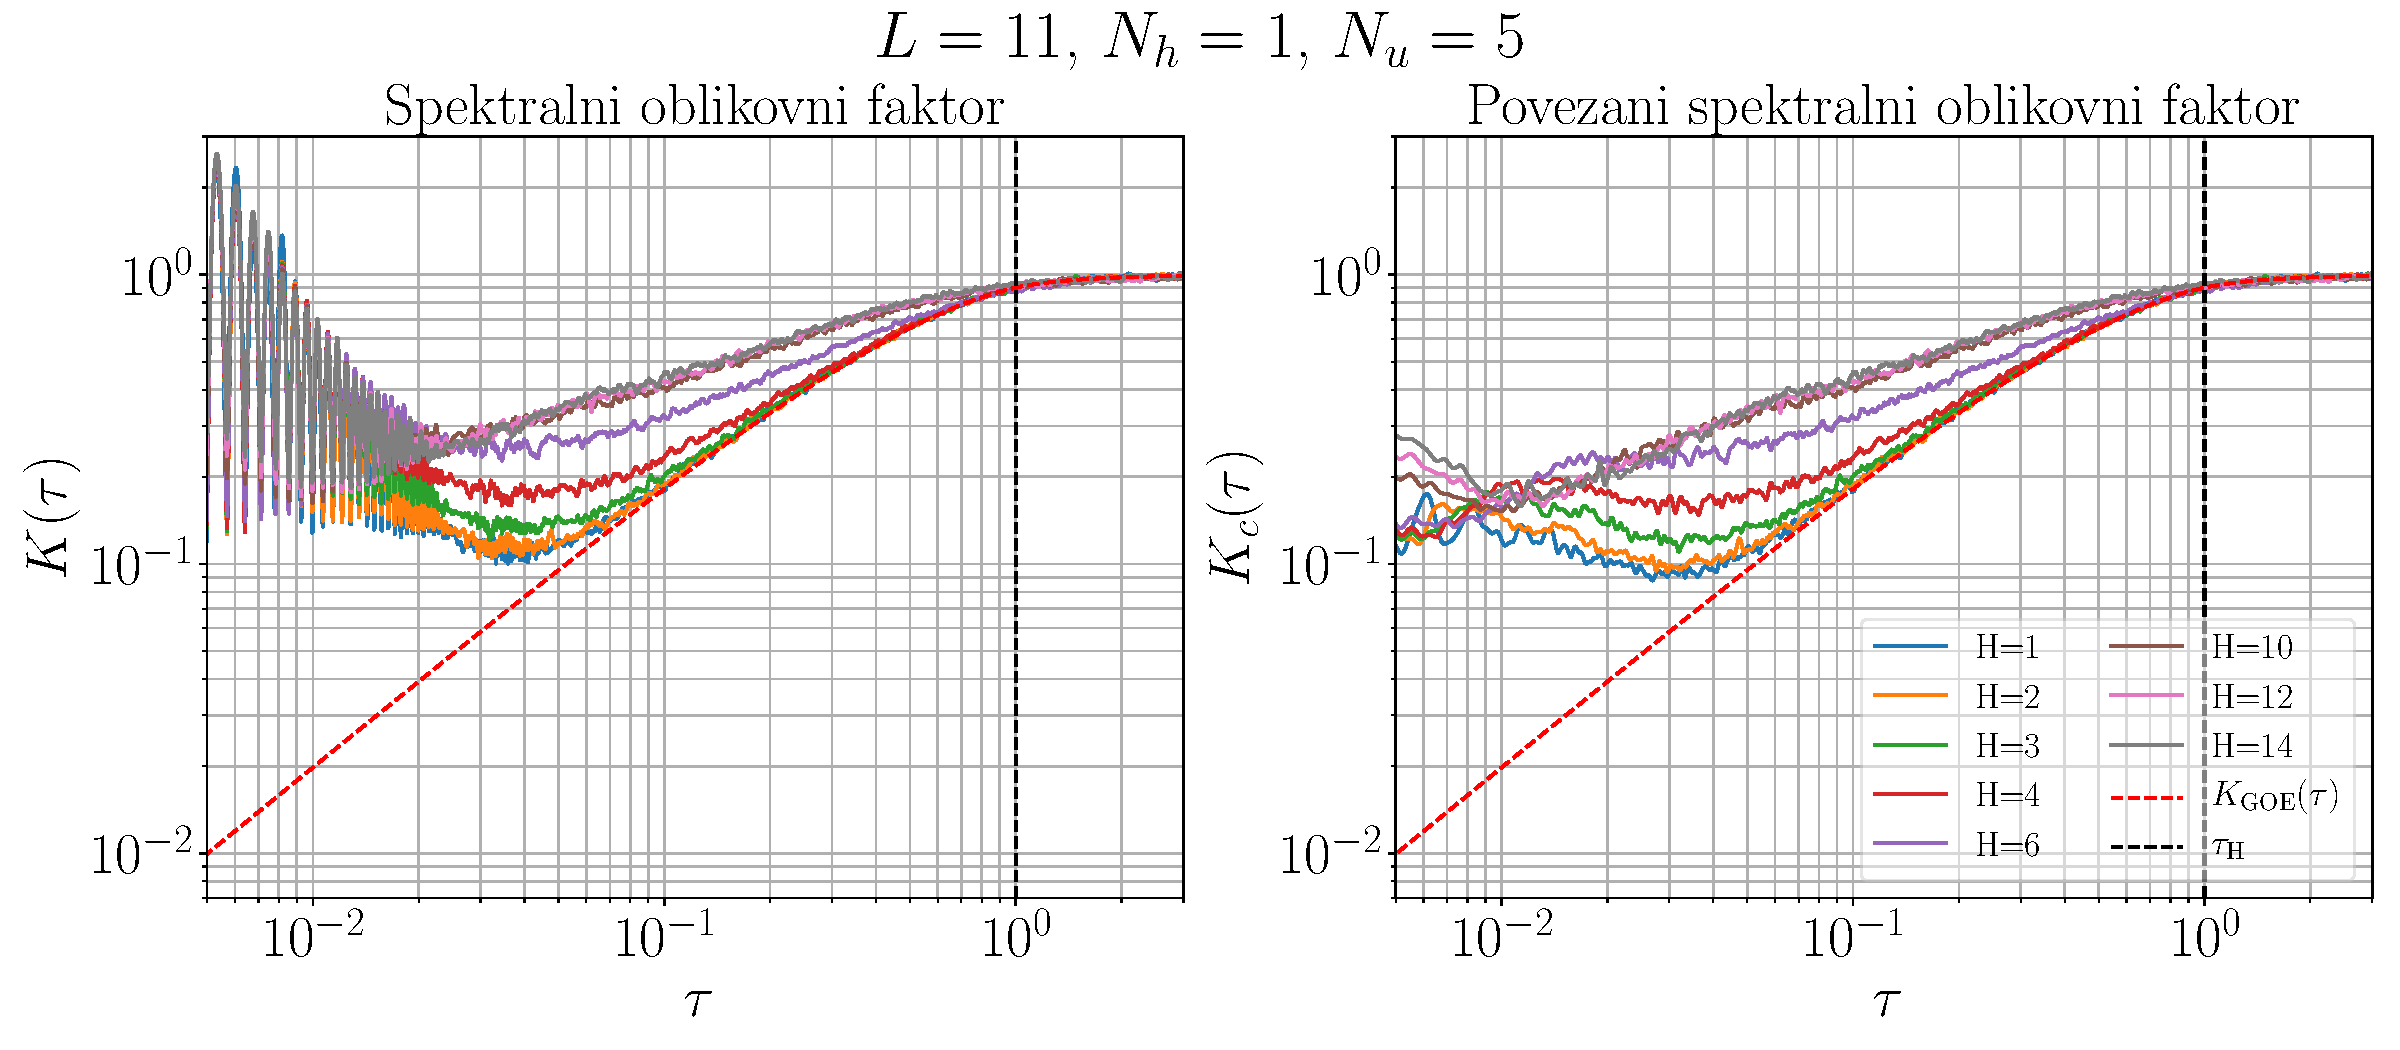
\includegraphics[trim=570 2 0 33,clip,width=1\textwidth]{H_sweep_sff_disorder_11_1_5.pdf}}
% \caption{Vrzelni nered - \textbf{ni MBL}.}
% % \label{fig:scheme_sff_disorder_14_0_7}
% \end{figure} 
% \end{minipage}
% }
% \only<2>{\textbf{Za vrzelni nered NI PREHODA - vmesno obnašanje.}}
\only<1,2>{
Tretjinsko dopiranje - $L=9, N_h=3, N_u=3$\vspace{7mm}
\begin{minipage}[c]{0.48\textwidth}
\begin{figure}[H]
\centering{
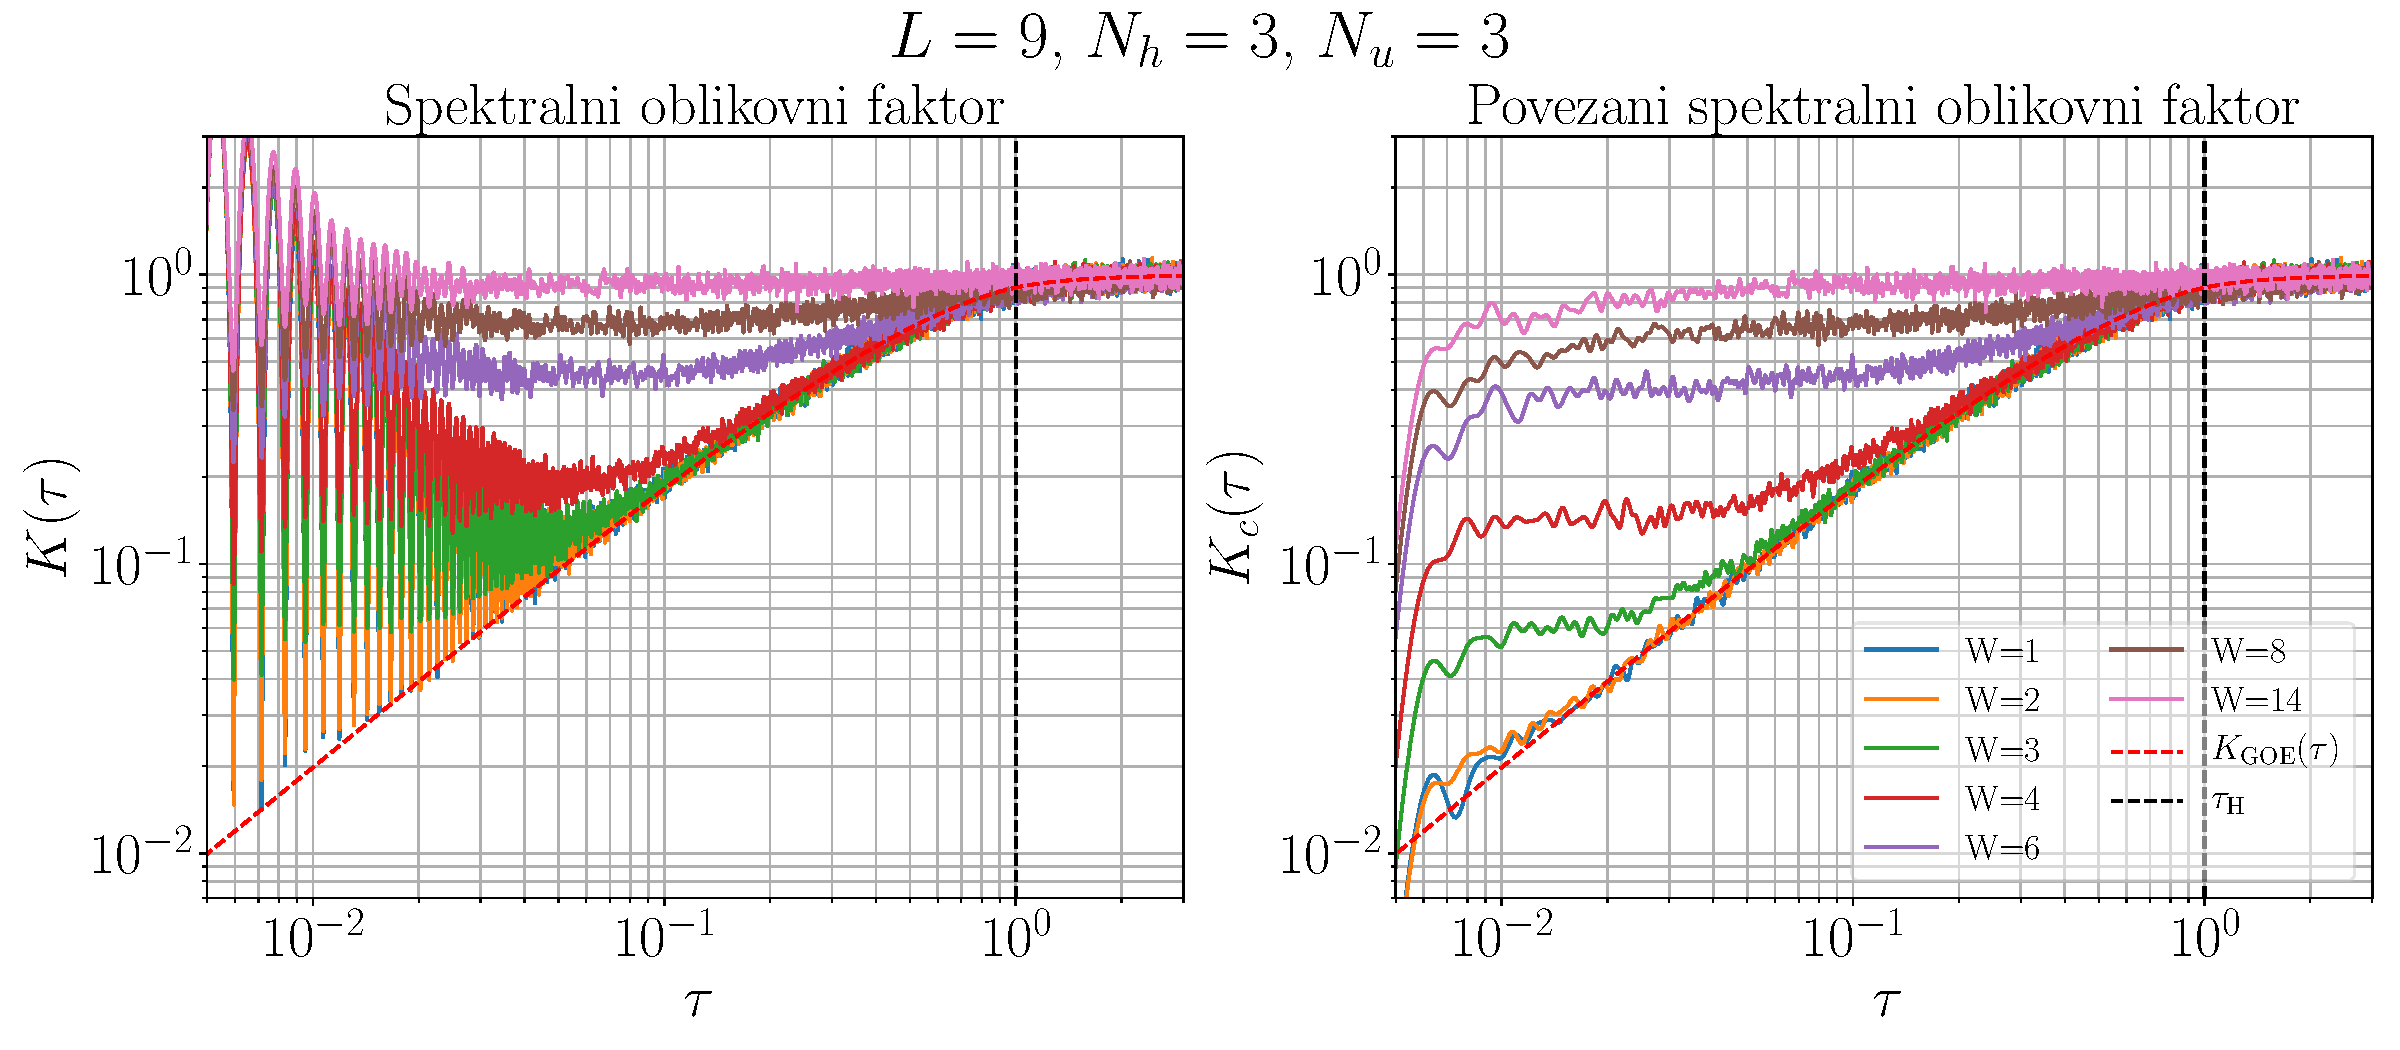
\includegraphics[trim=570 0 0 33,clip,width=1\textwidth]{W_sweep_sff_disorder_9_3_3.pdf}}
\caption{Spinski nered.}
% \label{fig:scheme_sff_disorder_14_0_7}
\end{figure} 
\end{minipage}\hfill
\begin{minipage}[c]{0.48\textwidth}
\begin{figure}[H]
\centering{
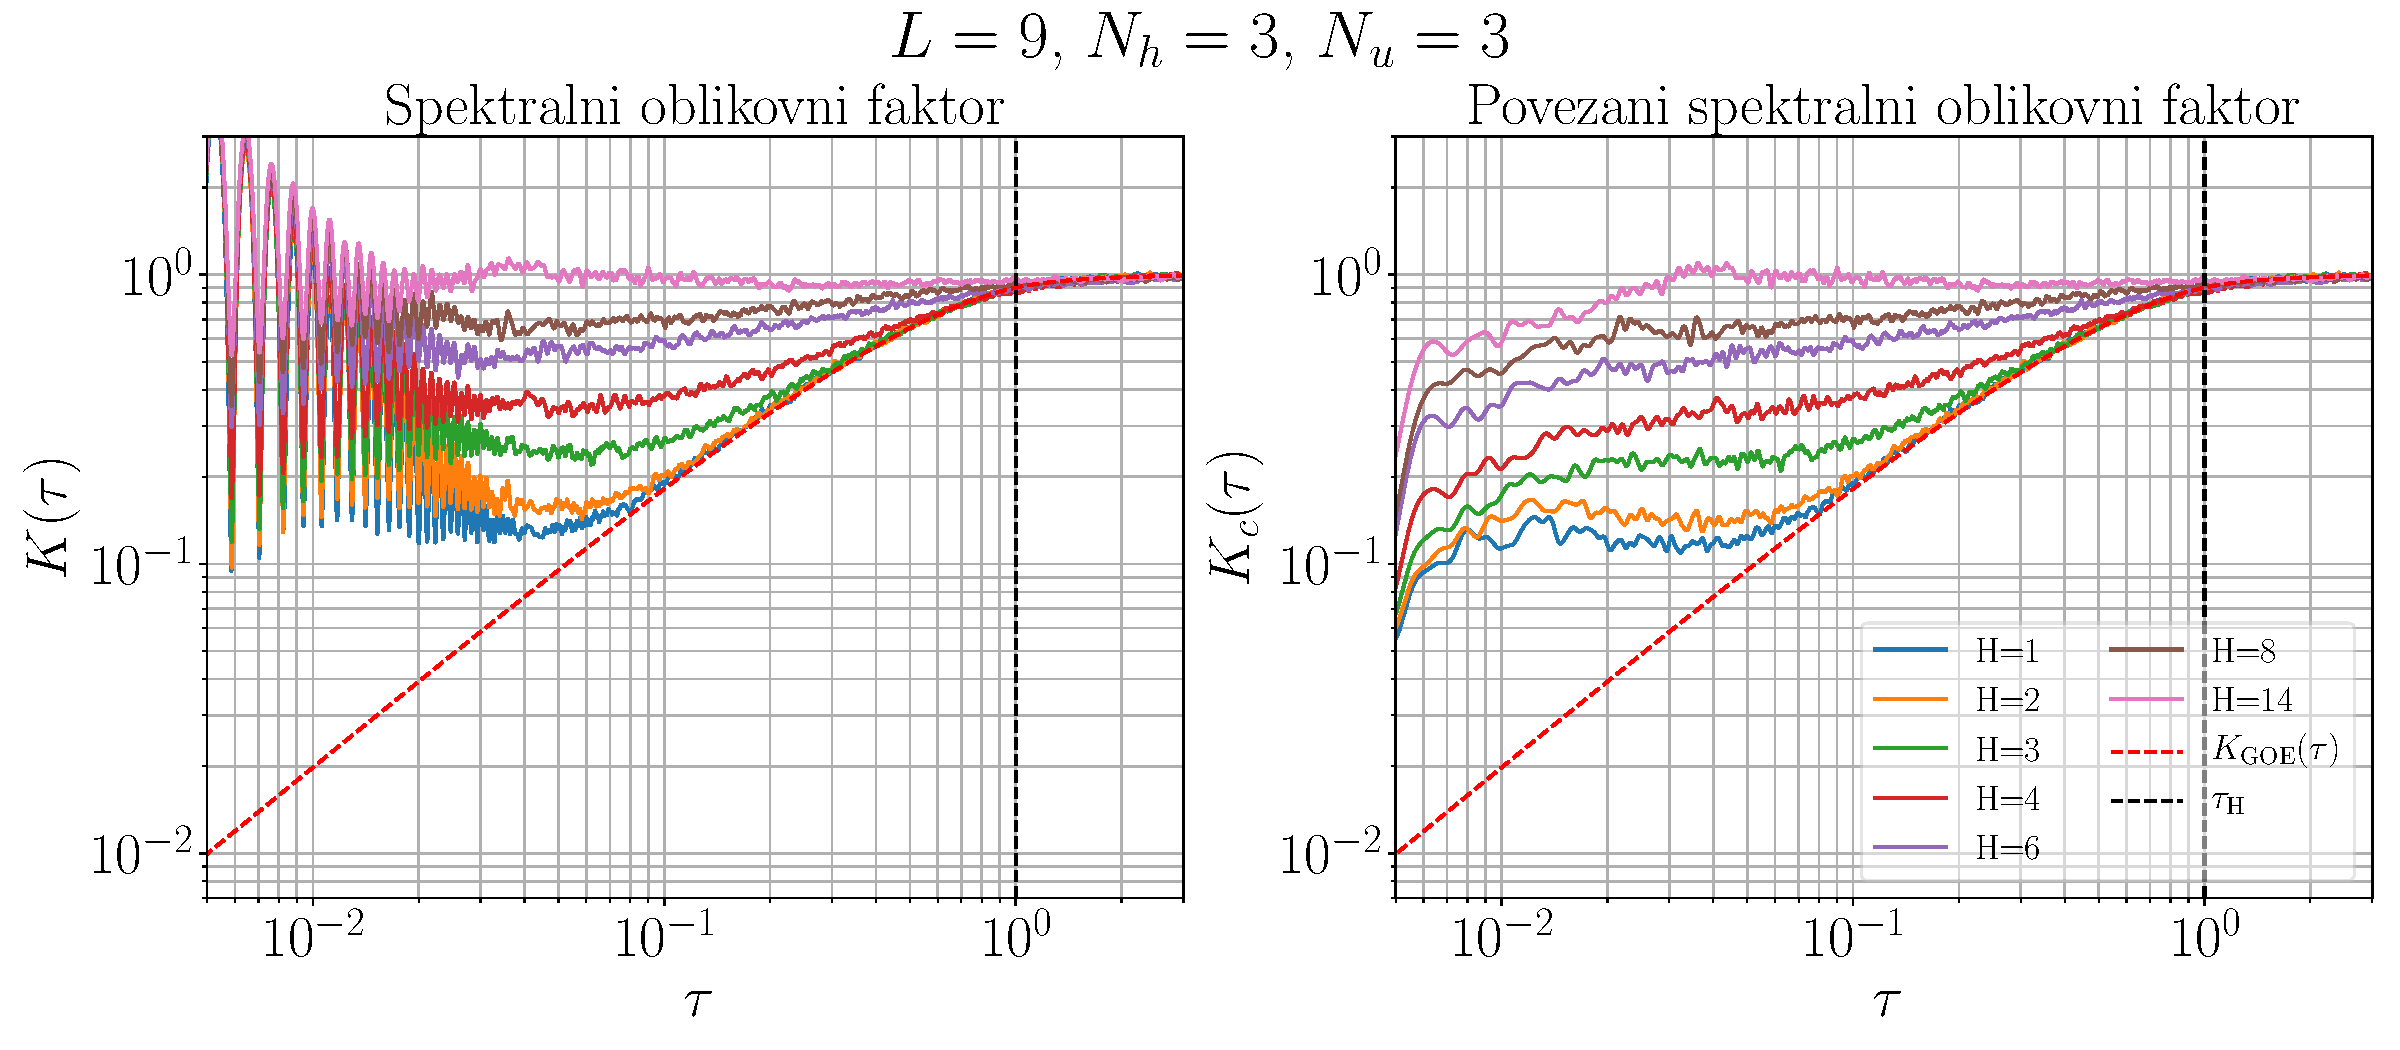
\includegraphics[trim=570 2 0 33,clip,width=1\textwidth]{H_sweep_sff_disorder_9_3_3.pdf}}
\caption{Vrzelni nered.}
% \label{fig:scheme_sff_disorder_14_0_7}
\end{figure} 
\end{minipage}
}
\only<2>{\textbf{Prehod v MBL za oba tipa nereda.}}

\end{frame}

\begin{frame}{Prepletenostna entropija}
\only<1,2>{
Računamo: Prepletenostno entropijo \textbf{VSEH} lastnih stanj.\\\vspace{5mm}
Sistem razdelimo na \textbf{podsistema} A in B.\vspace{5mm}}
\only<1>{
	
\begin{figure}[H]
\centering{
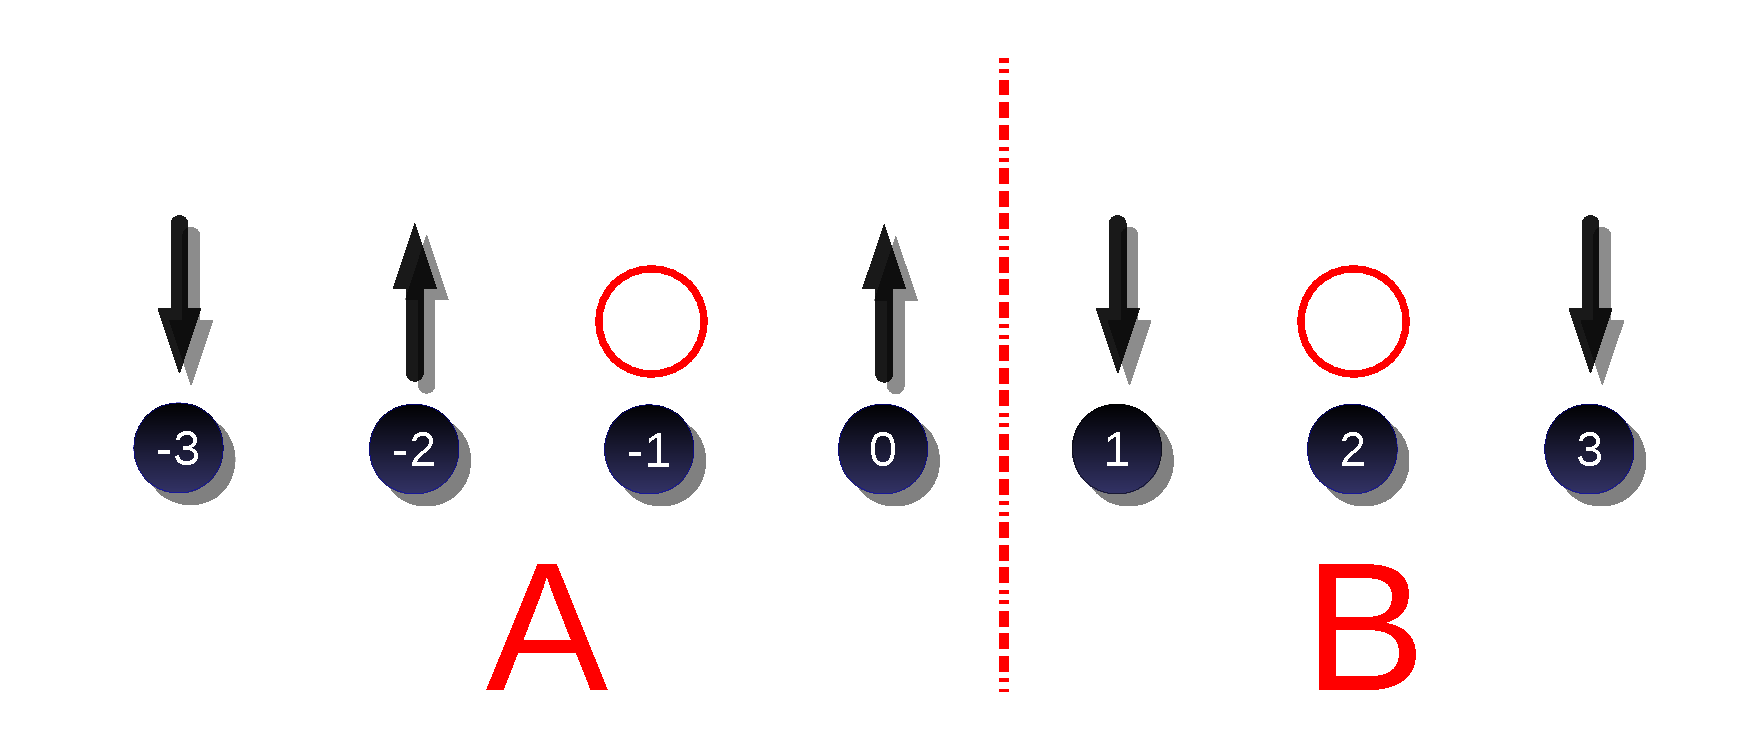
\includegraphics[width=0.7\textwidth]{tJ_scheme_bipartition.pdf}}
% \caption{Vrzelni nered.}
% \label{fig:scheme_sff_disorder_14_0_7}
\end{figure}
}
\only<2>{
\begin{alertblock}{\centering{Reducirana gostotna matrika podsistema:}}
$$
\rho_\mathrm{A} = \mathrm{Tr}_\mathrm{B} \rho, \hspace{5mm} \rho = \ket{\psi}\bra{\psi}
$$
\end{alertblock}\vspace{7mm}

\begin{alertblock}{\centering{Prepletenostna entropija - von Neumannova entropija podsistema}}
$$
S_\mathrm{ent}(\mathrm{A})=-\Tr\left\{\rho_\mathrm{A} \log \rho_\mathrm{A}\right\}=-\sum\limits_{i=1}^{d_\mathrm{A}} \lambda_i^\mathrm{A} \log \lambda_i^\mathrm{A} 
$$
\end{alertblock}}


\only<3>{
\begin{minipage}[c]{0.34\textwidth}
Volumsko skaliranje:
$$S_\mathrm{A}\propto L_\mathrm{A}, \hspace{3mm} L\to\infty$$
Površinsko skaliranje:
$$S_\mathrm{A}/L=\mathrm{const.}, \hspace{3mm} L\to\infty$$
\end{minipage}}\hfill
\only<3,4>{
\begin{minipage}[c]{0.62\textwidth}
\begin{figure}[H]
\centering{
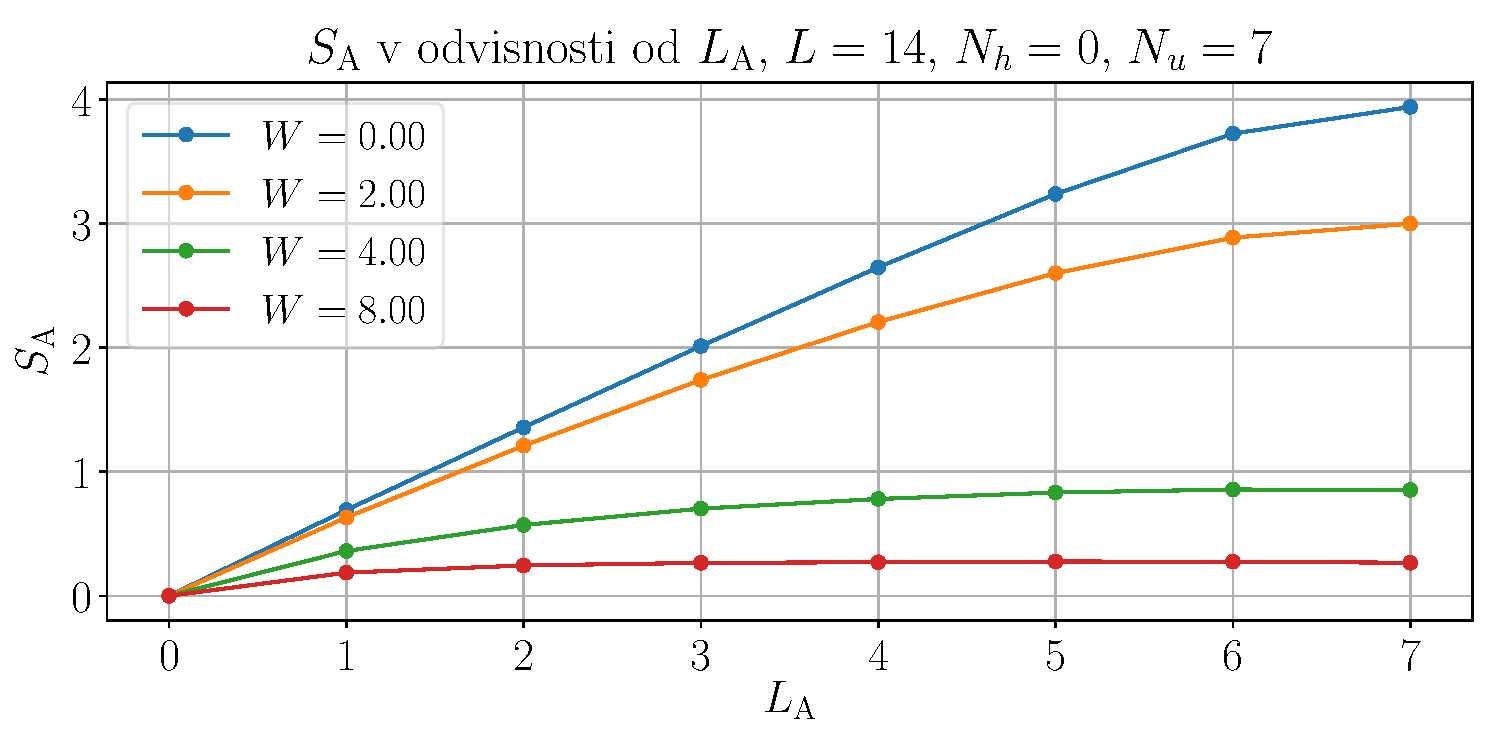
\includegraphics[width=1\textwidth]{W_sweep_ent_entropy_scaling_14_0_7.pdf}}
\end{figure}
\end{minipage}}\\
\only<4>{
\begin{minipage}[c]{0.34\textwidth}
Volumsko skaliranje:
$$S_\mathrm{A}/L=\mathrm{const.}, \hspace{3mm} L\to\infty$$
Površinsko skaliranje: 
$$S_\mathrm{A}/L\to 0, \hspace{3mm} L\to\infty$$
\end{minipage}}\hfill
\only<3,4>{
\begin{minipage}[c]{0.62\textwidth}
\begin{figure}[H]
\centering{
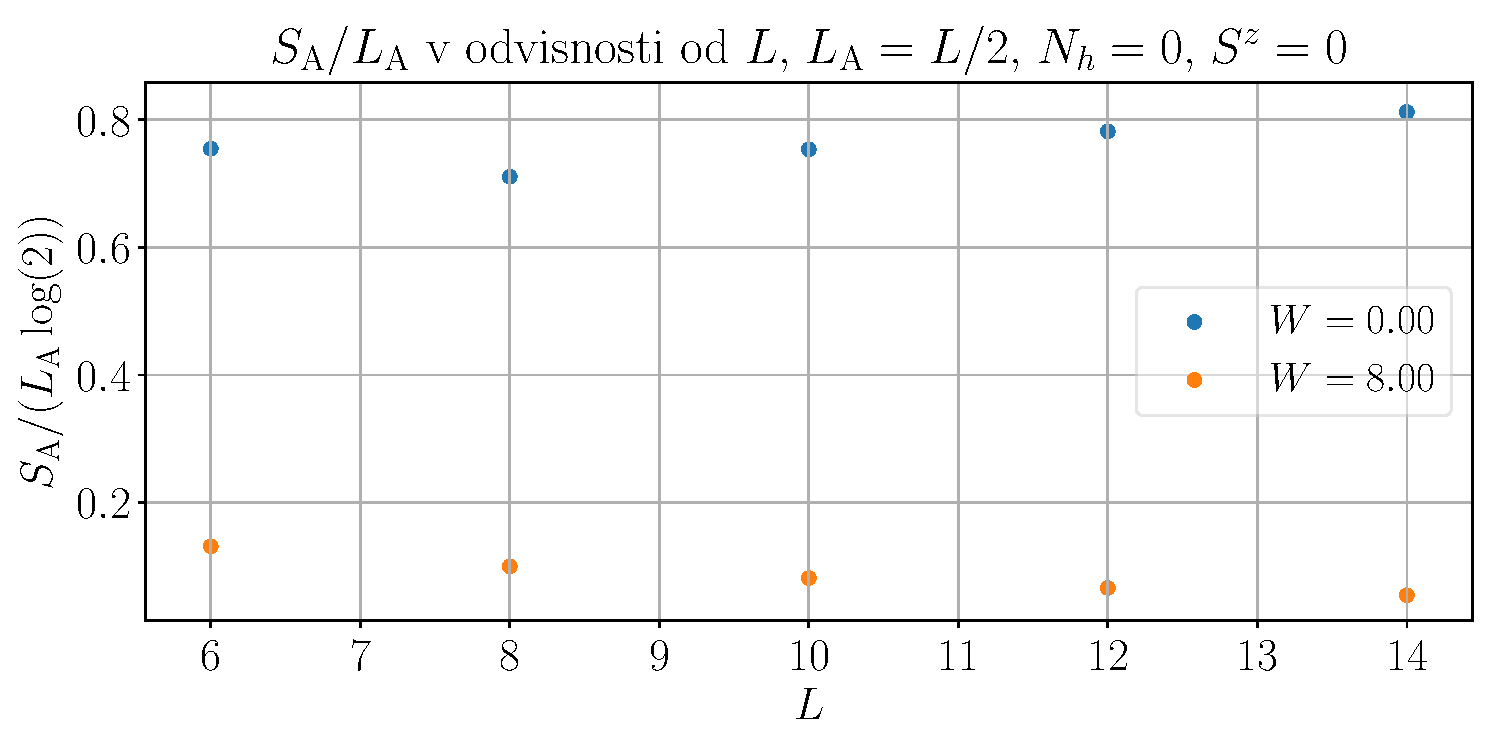
\includegraphics[width=1\textwidth]{W_sweep_ent_entropy_scaling_systems_14_0_7.pdf}}
% \caption{Vrzelni nered.}
% \label{fig:scheme_sff_disorder_14_0_7}
\end{figure}
\end{minipage}}
\end{frame}

\begin{frame}{Prepletenostna entropija - rezultati}
% \only<1,2>{
% \begin{figure}[H]
%  \centering{
% 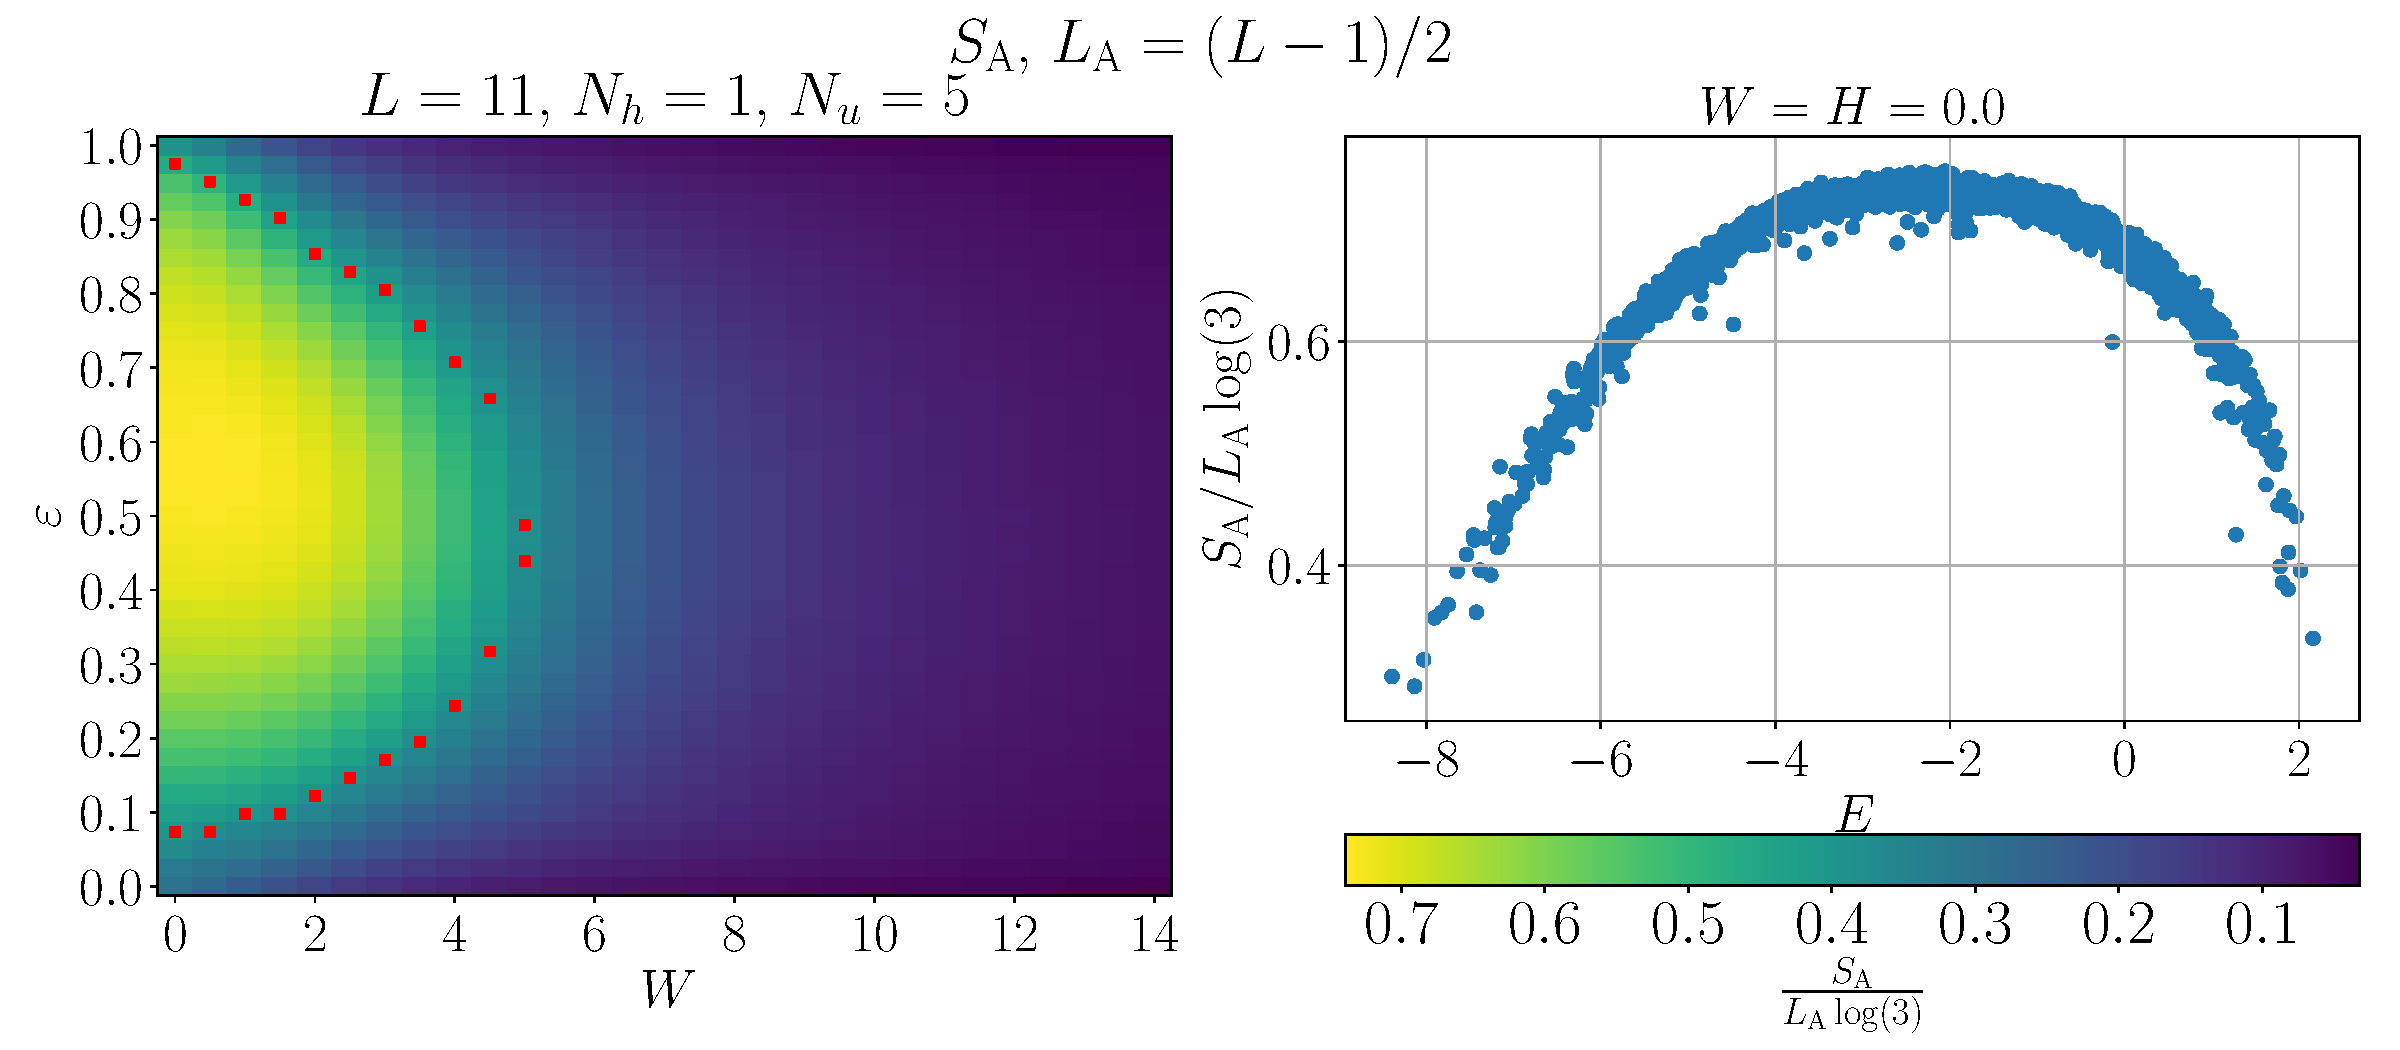
\includegraphics[width=0.65\textwidth]{W_sweep_ent_entropy_density_plot_11_1_5_cuts.pdf}}
% \end{figure}}
% \only<2>{
% \begin{minipage}[c]{0.4\textwidth}

% Ena vrzel, vrzelni nered:\\
% \centering{\textbf{ne vidimo prehoda}}
% \end{minipage}}
% \only<1,2>{
% \begin{minipage}[c]{0.4\textwidth}
% \begin{figure}
% \centering{
% 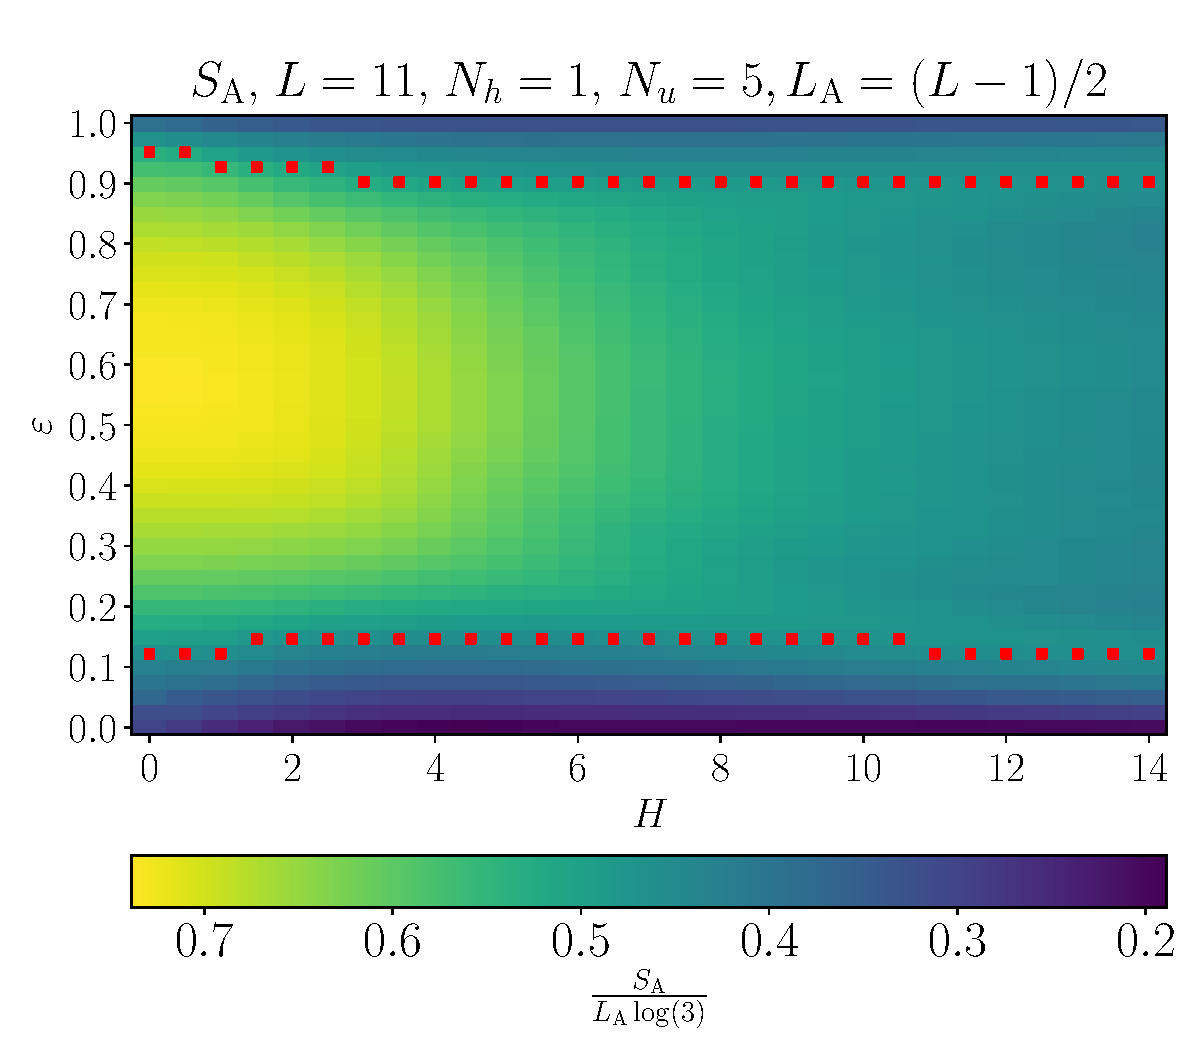
\includegraphics[width=1\textwidth]{H_sweep_ent_entropy_density_plot_11_1_5.pdf}}
% % \caption{672 citations as of April 2018 acc. to Google Scholar.}
% \end{figure}
% \end{minipage}}
\only<1>{
\begin{figure}[H]
 \centering{
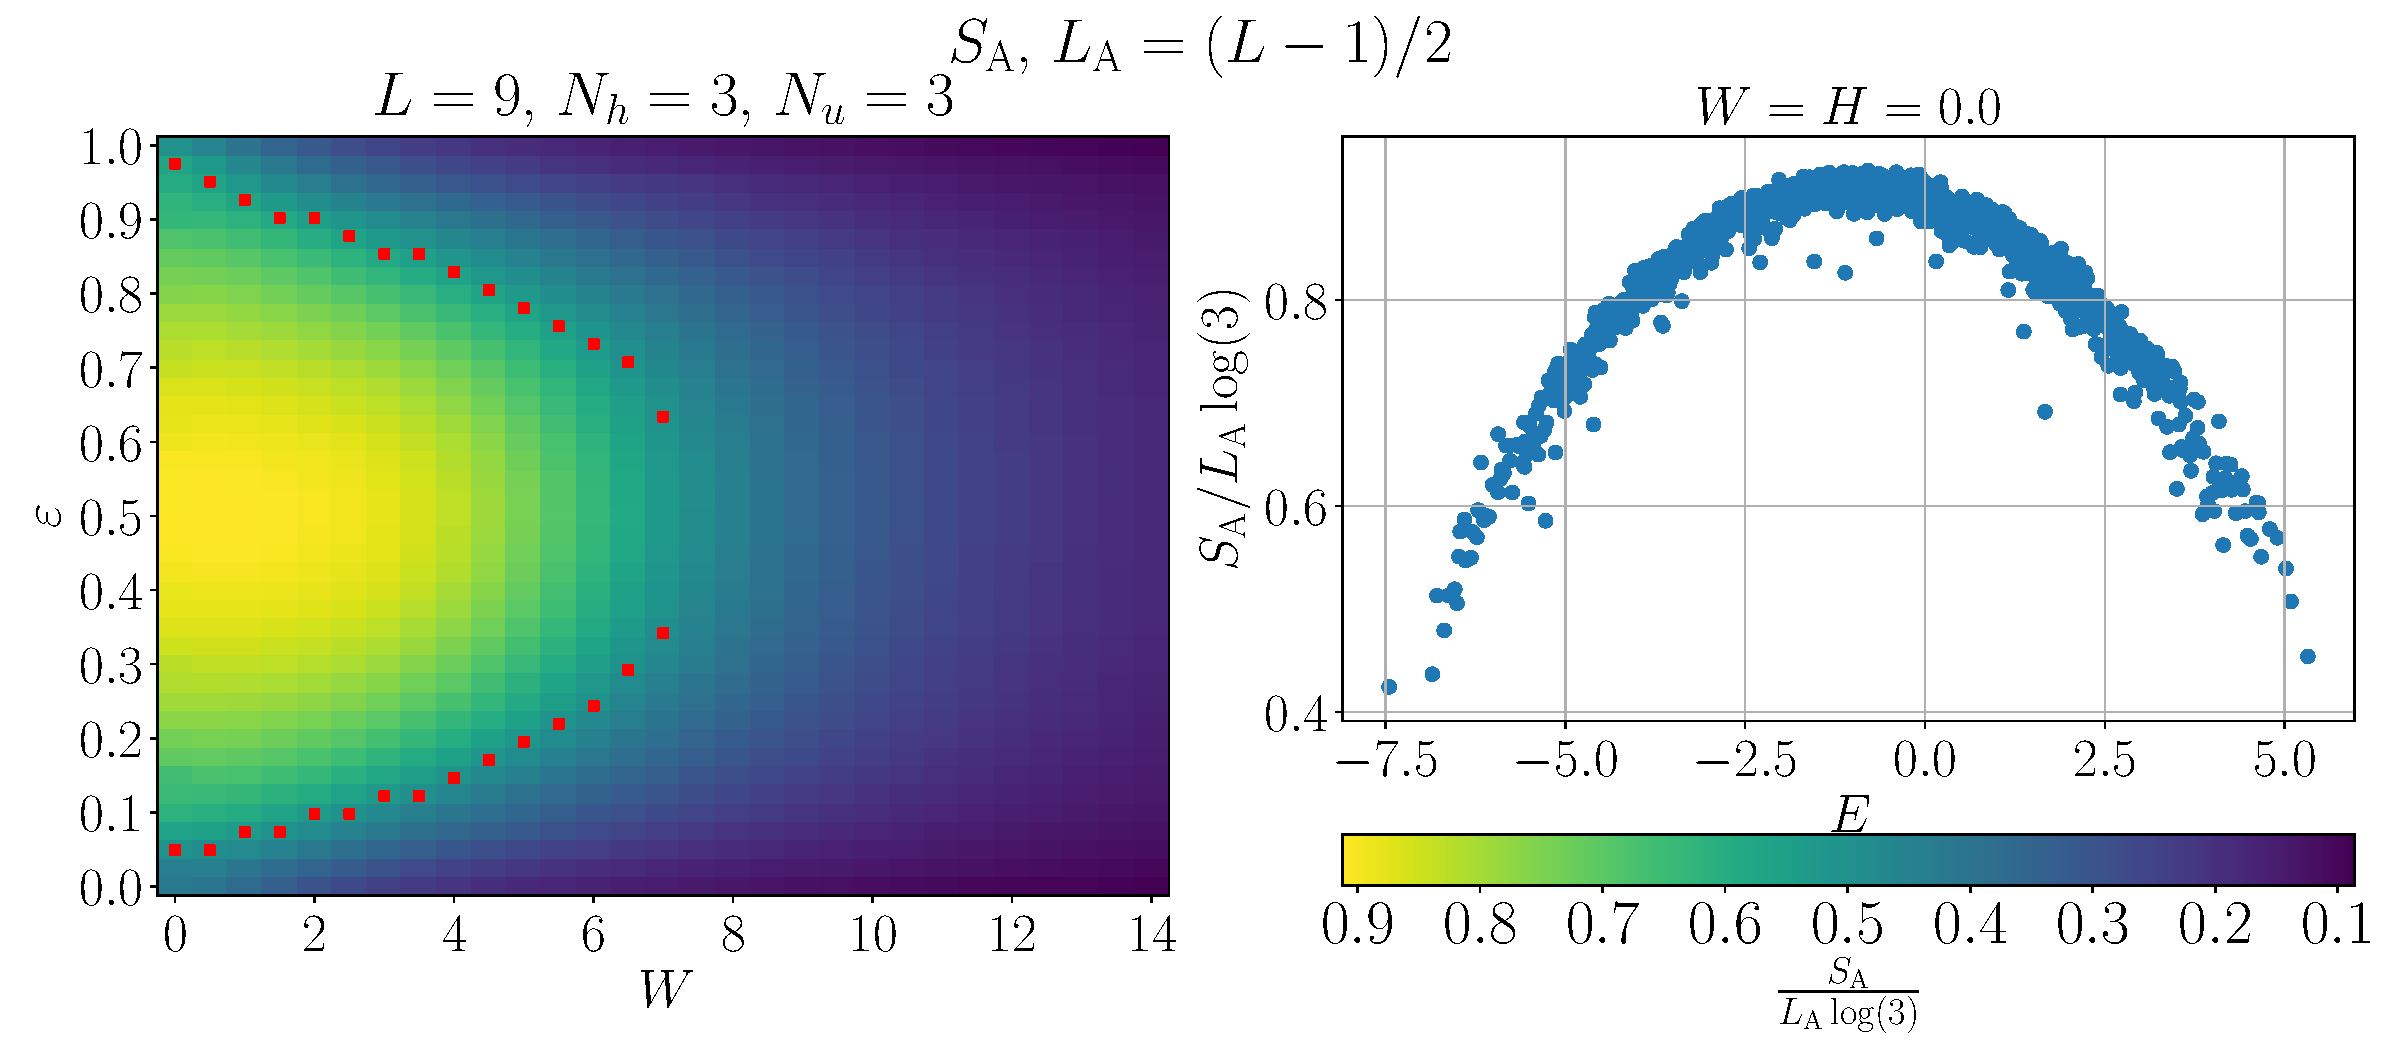
\includegraphics[width=0.65\textwidth]{W_sweep_ent_entropy_density_plot_9_3_3_cuts.pdf}}
\centering{
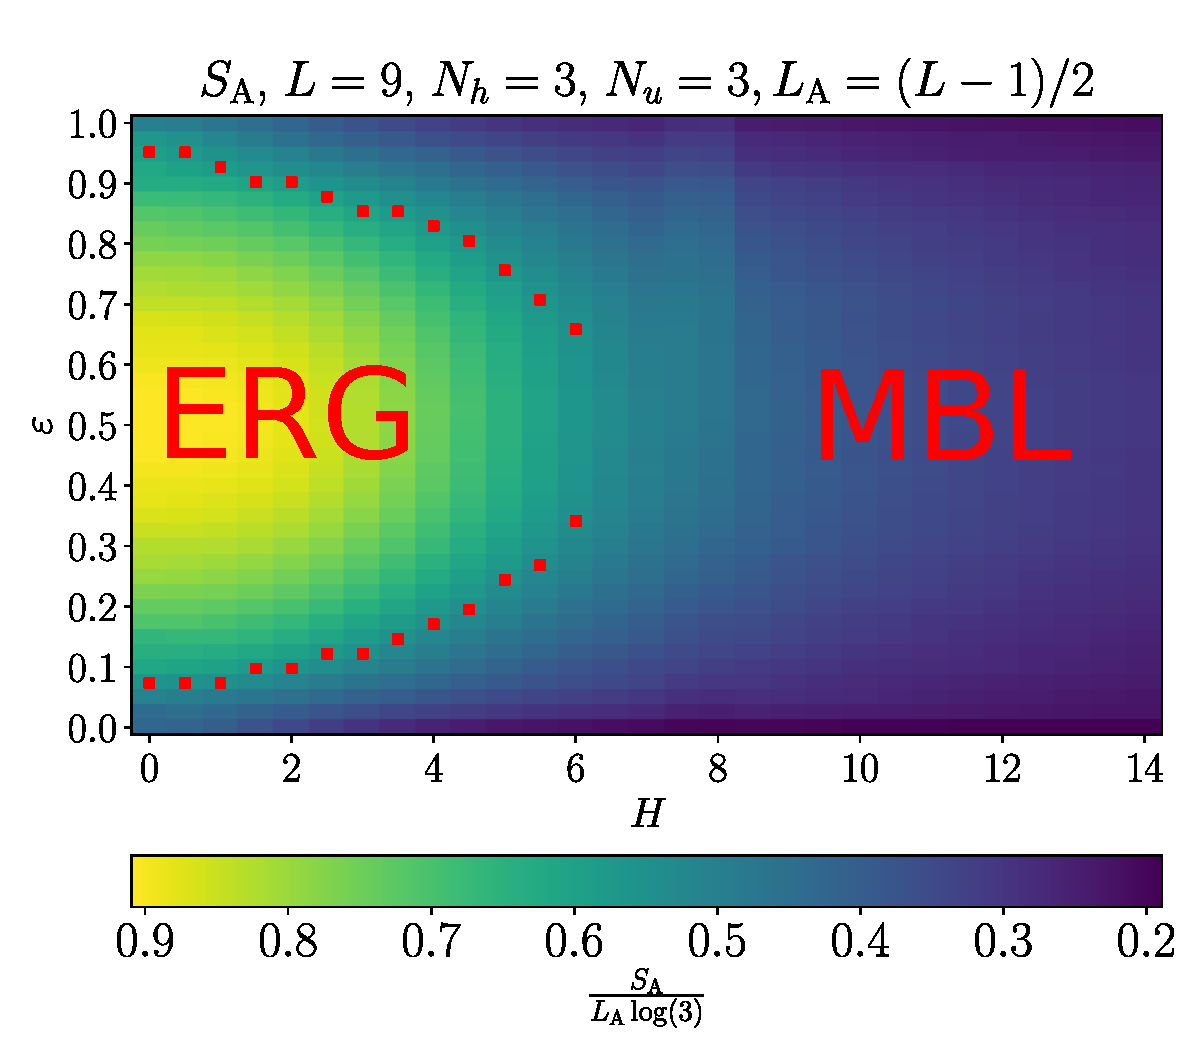
\includegraphics[width=0.4\textwidth]{H_sweep_ent_entropy_density_plot_9_3_3.pdf}}
\end{figure}}

\end{frame}


\begin{frame}{Zaključek}
\only<1>{
\begin{enumerate}
	\item Končno dopiranje - nastop MBL za oba tipa nereda\vspace{10mm}
	\item Ujemajoče se napovedi treh različnih indikatorjev \vspace{10mm}
	\item Implementacija SFF odpira nove raziskovalne možnosti 
\end{enumerate}}
\only<2>{ Hvala za pozornost!}

\end{frame}

\end{document}


